\newpage
\section{Umsetzung}

%todo - Das Kapitel Umsetzung sollte noch ein Kapitel/Absatz hervorgehen wo die Anforderungen erleutert werden - der erste satz von Kapitel 4 ist was kurz. 4.1 ist ok, aber, danach fehlt dann design von labels. 
In dieser Arbeit wird angestrebt, Objekte einer AR-Umgebung zu erkennen und mit Labels zu versehen.  RGB-Bilder der Umgebung werden aufgenommen und von neuronalen Netzen nach Objekten durchsucht. Gefundenen Objekte werden in einer 3D-Rekonstruktion der Umgebung lokalisiert und mit Labels markiert. Durch diesen Vorgehen können Objekte der Umgebung automatisch erkannt und mit Labels ausgestattet werden.

\subsection{Anforderungen}
%todo read this over. it is new
Die Objekterkennung und das Setzten der Labels soll ohne Zutun eines menschlichen Nutzers ablaufen. Der Vorgang braucht nicht in Echtzeit zu geschehen. Er soll jedoch eine Laufzeit haben, welche das Labeln eines Raumes binnen 10 Minuten erlaubt.

Objekte werden anhand des Mittelpunktes ihrer Bounding-Box markiert. Die Foto-Position des Objektes soll möglichst genau auf die 3D-Szene übertragen werden. An die berechnete 3D-Position der Szene wird ein Label gesetzt, welches die Klasse des Objektes wiedergibt. Jedes Objekt wird durch maximal ein Label annotiert. Wenn ein Objekt mehrmals erkannt wird, soll kein neues Labels in der Szene erzeugt werden. Die Applikation soll erkennen, dass das Objekt bereits durch ein Label markiert ist.

Die Applikation soll über ein minimales View Management verfügen. Die Labels werden als 3D-Objekte dort in der Szene platziert, wo das entsprechende Objekt lokalisiert wurde. Dabei wird nicht darauf geachtet, ob sie andere Labels oder reale Gegenstände verdecken. Wenn der Nutzer sich in der Szene bewegt, sollen die Labels nachgeführt werden, damit der Schriftzug der Labels jederzeit dem Nutzer zugewandt ist.

%Label setzung ohne zutun eines menschen. keine Echtzeit. Labels abspeichern. Labels präzise platzieren, so wie durch Fotos erkannt wurde. Labels auch wenn man sich in der Szene bewegt noch lesen können. Labels markieren den Mittelpunkt des jeweiligen Objektes. Keine Doppelten erkennung desselben objektes. Mit möglichst wenigen Bildern semantische Information erhalten

\subsection{Design der Objekternennung}

Im Folgenden werden die Arbeitsschritte einer Objekterkennung beschrieben.

Wenn der Nutzer das Signal gibt, beginnt die Detection. Als Erstes wird ein Foto mit der Kamera der AR-Brille aufgenommen. Dieses Foto wird an Azure Object Detection und Azure Custom Vision geschickt.
Die beiden Services untersuchen das Foto nach Objekten, um deren Klassen und Positionen auf dem Foto anzugeben.

Für jedes Objekt soll ein Label erstellt werden, welches zeigt, wo sich das Objekt in der realen Welt befindet.
Dafür wird in der 3D-Szene der AR-Umgebung eine virtuelle Repräsentation des Fotos erschaffen. Diese Fotorepräsentation muss sowohl die korrekte Skalierung als auch die korrekte Position und Rotation haben, um das räumliche Verhältnis zwischen der realen Fotokamera und der Umgebung nachbilden zu können.

Da die Fotokamera und das Display nahe beieinander liegen und den gleichen Blickwinkel haben, kann die Position des Displays als Repräsentation des Fotos genutzt werden. In der 3D-Szene ist das Display mit der Hauptkamera gleichgesetzt. Die Clipping Plane der Kamera hat somit die gleiche Rotation und eine zumindest ähnliche Position und Skalierung wie das Foto. Daher werden die Foto-Positionen auf Koordinaten der Clipping Plane abgebildet. Dabei werden verbleibende Positions- und Skalierungsunterschiede ausgeglichen. Für jedes Objekt wird so eine Position auf der Clipping Plane bestimmt.

Als Nächstes wird ein Raycast von der Kamera aus durch die Clipping Plane Position geschickt. Der Raycast schneidet sich mit einem Mesh, welches die reale Welt abbildet. Die getroffene Position wird mit einem Label markiert. Dort befindet sich das Objekt, welches auf dem Foto gefunden wurde. Alle Objekte, die Azure Object Detection und Azure Custom Vision gefunden haben, werden so für den Nutzer in der AR-Umgebung markiert.

\subsection{Design der Labels}
%todo this is new

Die Labels der erkannten Objekte werden als 3D-Objekte in der Szene platziert. Sie bestehen aus einer Sphäre (Anchor) und einem Schriftzug. Die Sphäre liegt an der 3D-Position des Objektes. Der Schriftzug befindet sich über der Sphäre. Er gibt die Klasse des Objektes wieder, welches durch ein neuronales Netzwerk erkannt wurde.

Um sicherzustellen, dass Objekte durch maximal ein Label annotiert werden, wird jedes Mal, wenn ein Label in der Szene platziert werden soll, überprüft, welche Labels sich in der Nähe befinden. Gibt es bereits ein Label mit demselben Schriftzug, wird davon ausgegangen, dass es sich auf dasselbe Objekt der realen Welt bezieht. Ein Gegenstand wurde demnach zweimal erkannt. Aus den beiden Objekterkennungen gehen zwei 3D-Positionen hervor, die für das Objekt lokalisiert werden. 

Beide 3D-Positionen werden jeweils mit einem 3D-Objekt markiert. Das Label des Objektes wird in den Mittelpunkt der Positionen gesetzt. Fall das Objekt öfter als zwei Mal erkannt wird, erfolgt die Markierung aller 3D-Positionen, welche durch die Objekterkennungen bestimmt wurden. Das Label sitzt in der Mitte aller lokalisierten Positionen.

Wenn der Nutzer sich in der Szene bewegt, rotieren die Labels sich um ihre Anchor, damit der Schriftzug dem Nutzer immer zugewandt bleibt.

Die Labels werden in einer Unity-Szene als GameObjects umgesetzt. Letzteren wird über Components die beschriebene 3D-Form der Labels gegeben, die von der Unity-Kamera gerendert wird. Die gerenderten Frames werden von dem Display der Magic Leap Brille angezeigt. 

\subsection{Architektur}

Die AR-Brille 'Magic Leap One' übernimmt alle Berechnungen im 3D-Raum und führt Spatial Mapping durch. Da die Analyse von RGB-Fotos sehr speicher- und rechenintensiv ist, wird sie an eine REST-API delegiert. Die AR-Brille 'Magic Leap One' wird als Interaktionsmöglichkeiten für den Nutzer verwendet. Zudem nimmt sie die RGB-Fotos der Umgebung auf, liefert diese an die REST-API und zeigt die Ergebnisse und Zwischenstände der Objekterkennung mit UI-Elementen in der Szene an. Siehe Abbildung \ref{dia:flow}

\begin{figure}[H]
	\centering
	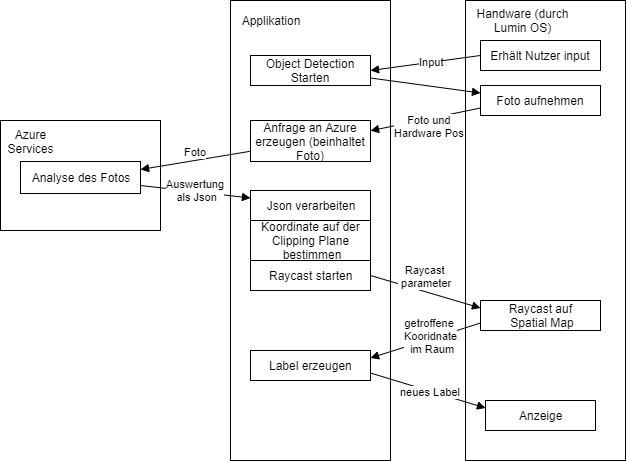
\includegraphics[width=1\textwidth]{images/dia_flow.png}
	\caption[Diagramm der Architektur]{Diagramm der Architektur inklusive Bearbeitungsschritte und Informationsweitergabe.}
	\label{dia:flow}
\end{figure}

% https://developer.magicleap.com/en-us/learn/guides/get-started-developing-in-unity
Die Arbeit wird mit der Entwicklungsumgebung Unity erzeugt. Als AR-Brille wird das Gerät 'Magic Leap One' verwendet. Für das Set-up des Unity-Projektes wird das Unity-Template von Magic Leap genutzt. Zusätzlich werden einige vorgefertigte Klassen von Magic Leap verwendet. Dazu gehören:  \textit{MLInput}, \textit{MLCamera}, \textit{MLRaycast}, \textit{MLPrivilegeRequestBehavior} und \textit{MLSpatialMapper}. Diese Klassen greifen auf Funktionalitäten des Betriebssystems Lumin OS zu.\citep{mlgetstarted}

Die benötigten Funktionalitäten für die Integration der Object Detection mit der REST-API werden in mehreren Script Klassen umgesetzt. Ein Großteil der Scripts verhält sich wie Singletons. Sie existieren nur einmalig in der Szene. Das Klassendiagramm auf Abbildung \ref{dia:classdiagramm} zeigt die Scripts und ihre Relationen zueinander.

\begin{figure}[H]
	\centering
	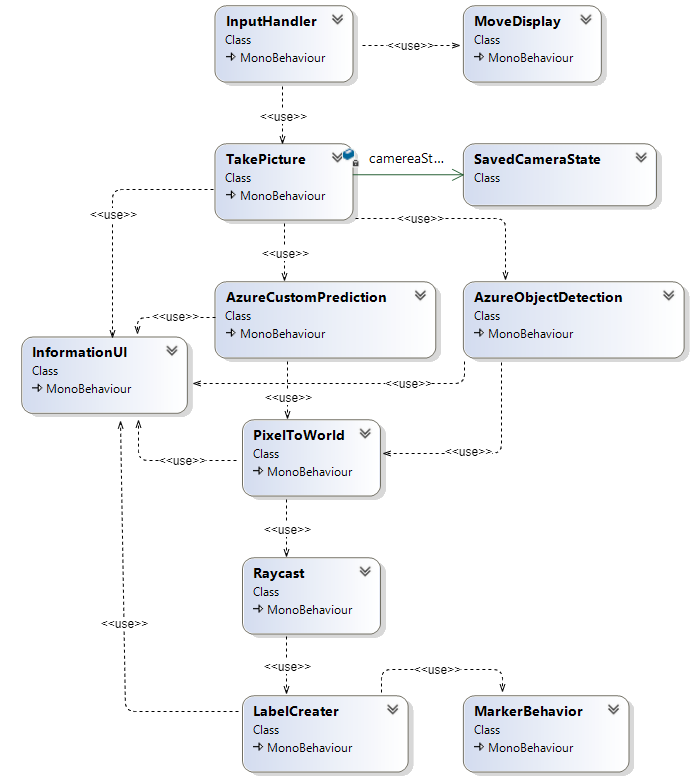
\includegraphics[width=1\textwidth]{images/klassendiagramm.png}
	\caption[Klassendiagramm der Skripts]{Klassendiagramme der Scripts}
	\label{dia:classdiagramm}
\end{figure}
 
Die Klassen \textit{InputHandler}, \textit{MoveDisplay}, \textit{LabelCreater}, \textit{InformationUI} und \textit{MarkerBehavior} sind für die Interaktion mit dem Nutzer zuständig. 

Die Klassen \textit{TakePicture}, \textit{SavedCameraState}, \textit{AzureCustomPredicton}, \textit{AzureObjectDetection} führen die Erkennung von Objekten anhand eines aufgenommenen Fotos durch. Die Klassen \textit{PixelToWorld} und \textit{Raycast} bestimmen eine Position für das Objekt in der 3D-Umgebung. Der Prozess wird durch den \textit{InputHandler} gestartet. 

Sobald ein Objekt erkannt und eine Position auf dem Mesh der Umgebung bestimmt wird, erfolgt der Aufruf von \textit{LabelCreater}. Diese Klasse erzeugt das Label des erkannten Objektes. Jedes Label wird als GameObject in der Unity-Szene erzeugt. Die Labels verfügen jeweils über ein  \textit{MarkerBehavior} Component. Mithilfe von \textit{MarkerBehavior} kann der Schriftzug des jeweiligen Labels angepasst werden.

\subsection{Interaktion}

Die Klasse \textit{InputHandler} verarbeitet den Input des Nutzers und startet entsprechende Aktionen durch die Klassen \textit{MoveDisplay} und \textit{TakePicture}. Der Input ist durch \textit{MLInput} abfragbar. Diese Klasse stellt Informationen über den Zustand des Controllers zur Verfügung. \textit{InputHandler} nutzt \textit{MLInput}, um den Controller zu überwachen. Wenn  Tasten des Controllers gedrückt werden, startet \textit{InputHandler} folgende Aktionen:

\begin{itemize}
	\item Trigger: Start der Objekterkennung mit \textit{TakePicture}
	\item Home Button: Mittige Platzierung des UI-Element vor dem Display
	\item Bumper: Verstecken der Labels
	\item Bumper halten: Entfernen des zuletzt erzeugten Labels
\end{itemize}

Das UI-Element wird von \textit{InformationUI} gesteuert. \textit{TakePicture} nutzt \textit{InformationUI}, um das zuletzt aufgenommene Foto anzuzeigen. \textit{AzureCustomPrediction}, \textit{AzureObjectDetection} und \textit{PixelToWorld} dokumentieren ihre Arbeitsschritte mit dem UI-Element. Der \textit{LabelCreater} zeigt eine Liste aller Labels an , die in der Szene existieren. Siehe Abbildung \ref{img:ausgabe}.

%\begin{figure}[H]
%	\centering
%	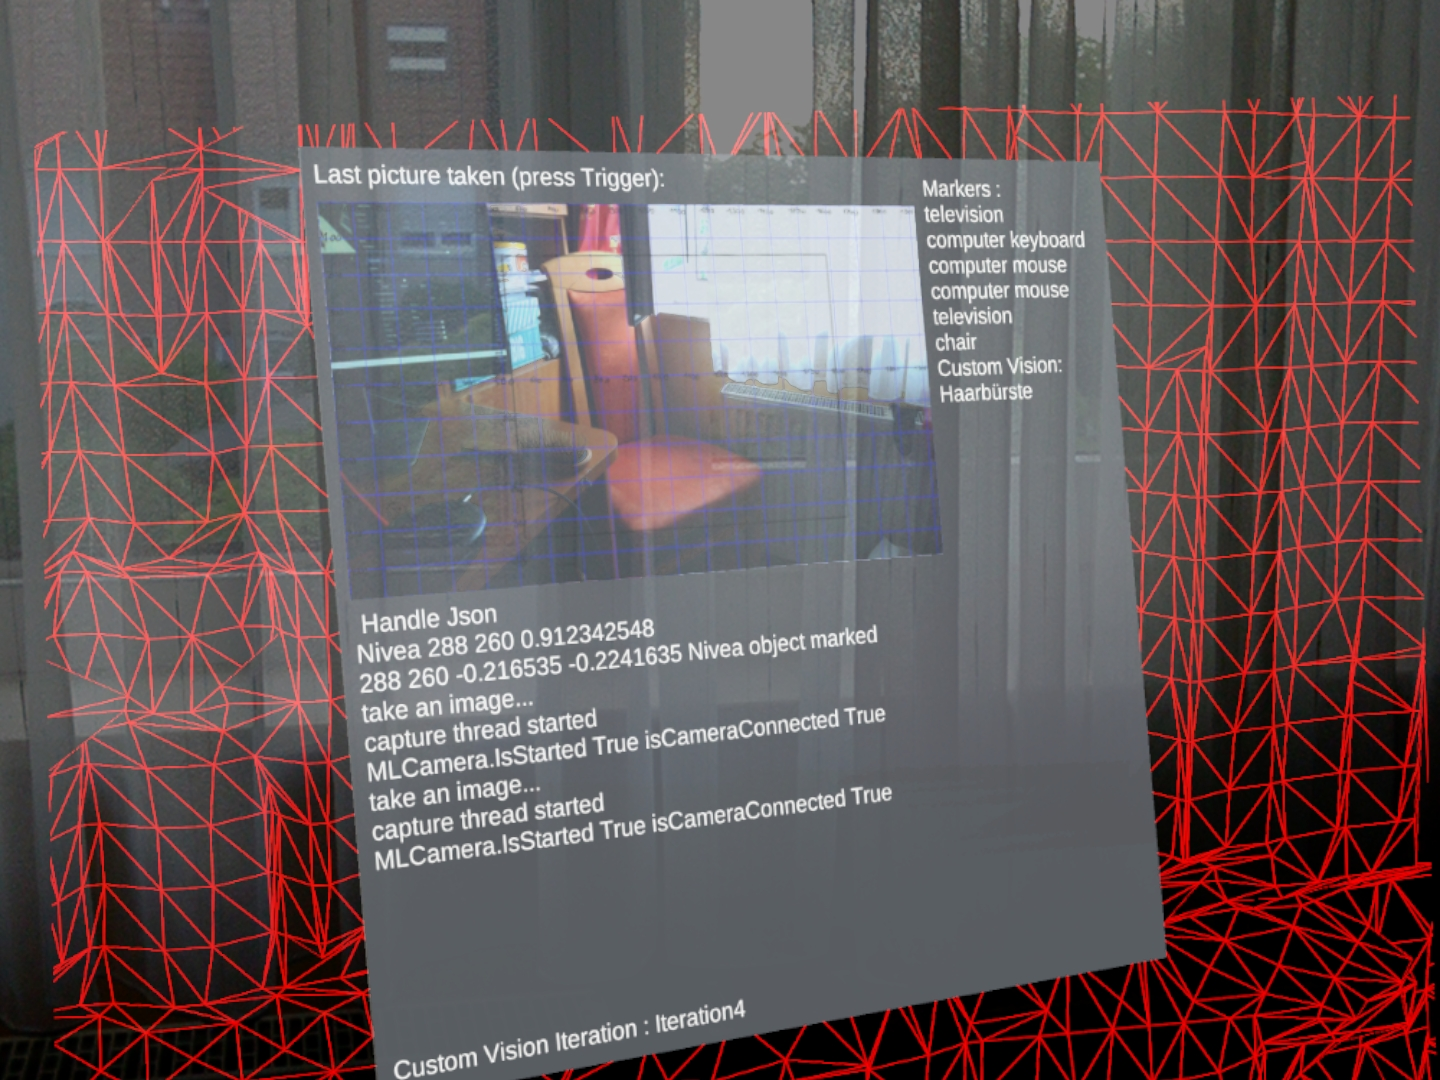
\includegraphics[width=1\textwidth]{images/ML_20200831_19.13.05.jpg}
%	\caption[]{UI Element}
%	\label{image:UIElement}
%\end{figure}

Der \textit{LabelCreater} ist für die Erstellung der Labels verantwortlich und sorgt dafür, dass die Labels für den Nutzer lesbar sind. Zu diesem Zweck werden die Labels in Richtung der Kamera ausgerichtet und mitgeführt. Des Weiteren kann der \textit{LabelCreater} Labels verstecken und entfernen.

Neben dem UI-Element und den Labels wird auch ein Mesh angezeigt, welches die Spatial Map der Umgebung wiedergibt. Das Spatial Mapping wird von dem Betriebssystem Lumin OS durchgeführt. Das Mesh wird durch die Klasse \textit{MLSpatialMapper} von Magic Leap erzeugt und angezeigt. Siehe Abbildung \ref{img:ausgabe}.

\begin{figure}[H]
	\centering
	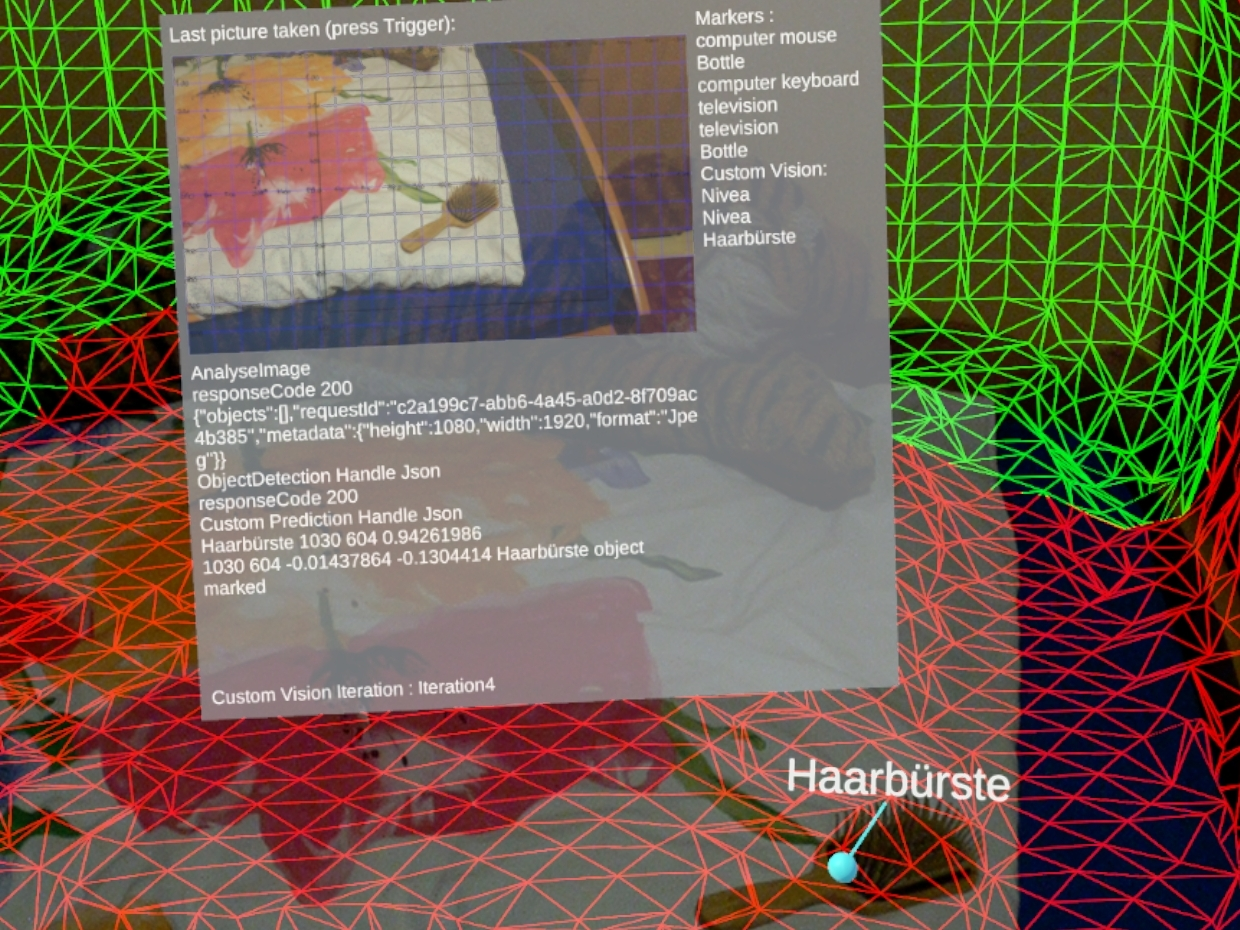
\includegraphics[width=0.9\textwidth]{images/ML_20201004_19.09.17_2.jpg}
	\caption[UI Ausgabe in der Szene]{Ausgabe}
	\label{img:ausgabe}
\end{figure}


\subsection{Implementierung der Objekterkennung}

Im Folgenden werden die Scripts besprochen, welche für die Objekterkennung zuständig sind.

\subsection{Ein Foto aufnehmen}

%\begin{figure}[H]
%	\centering
%	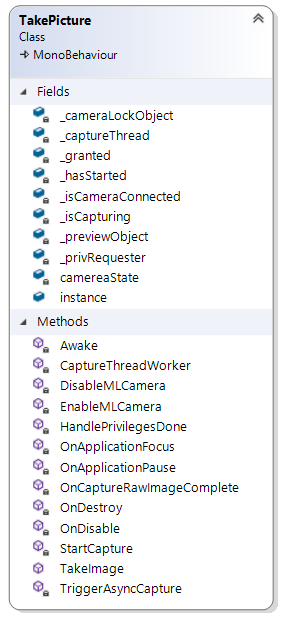
\includegraphics[width=0.4\textwidth]{images/dia_takepicture.PNG}
%	\caption[]{Klassendiagramm TakePicture}
%	\label{dia:takepicture}
%\end{figure} remake this image
%todo pause
Die Klasse \textit{TakePicture} implementiert die Aufnahme eines Fotos. Dabei wird \textit{MLCamera} von Magic Leap genutzt, um die Kamera der AR-Brille anzusteuern. Sobald die Applikation gestartet wird, stellt dieses Script sicher, das die Applikation die benötigte Permission hat, um die Kamera zu nutzen. Danach verbindet sich die Klasse über \textit{MLKamera} mit der Kamera-Ressource. Letztere wird wieder abgegeben, wenn die Applikation entweder terminiert oder pausiert wird.

Wenn die Methode \textit{TakeImage} aufgerufen wird, startet der Objekterkennung-Prozess.
Die Foto-Aufnahme geschieht asynchron. Für jedes Foto wird ein Thread erzeugt, in dem \textit{MLCamera} ein Foto aufnimmt. In diesem Thread wird zusätzlich die aktuelle Position der Unity Kamera als \textit{SavedCameraState} gespeichert.

Die Methode \textit{OnCaptureRawImageComplete} wird von \textit{MLCamera} aufgerufen, sobald das Foto fertig ist. Die Daten des Bildes und der \textit{SavedCameraState} werden, an die beiden Klassen \textit{AzureObjectDetection} und \textit{AzureCustomPrediction} weitergegeben. Diese führen Anfragen an die beiden Objekt Detection Services 'Azure Object Detection' und 'Azure Custom Vision' durch.

\subsubsection{Object Detection}

\begin{figure}[H]
	\centering
	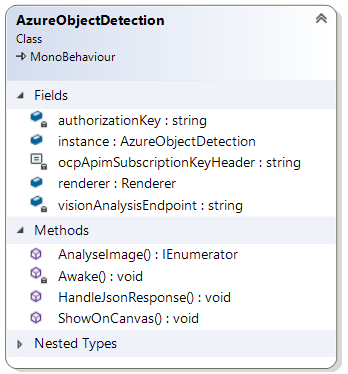
\includegraphics[width=0.5\textwidth]{images/dia_azureobjectdetection.PNG}
	\caption[Klassendiagramm von \textit{AzureObjectDetection}]{Klassendiagramm von \textit{AzureObjectDetection}}
	\label{dia:azureobjectdetection}
\end{figure}

In der Methode \textit{AnalyseImage} von \textit{AzureObjectDetection} wird ein Web Request zusammengestellt, um die Azure REST-API anzufragen. Der Request enthält eine Authentifizierung für die API und das zu analysierende Foto. %Siehe Abbildung \ref{dia:azureobjectdetection}.

Der Webrequest wird verschickt. Sobald die Antwort eintrifft, wird anhand des Response Codes geprüft, ob bei ein Fehler bei dem Request auftrat. Beispielsweise kann die Internetverbindung gestört sein oder die Authentifizierung abgelehnt werden. Wenn es keinen Fehler gab, wird eine Json-Datei bei der Antwort mitgeschickt. Darin wird für jedes gefundene Objekt auf dem Foto eine Bezeichnung und eine Bounding-Box angegeben. 

Die Json-Datei wird in \textit{HandleJsonResponse} verarbeitet. Für den erwarteten Aufbau der Datei gibt es drei Klassen: Der Json-String wird mit \textit{JsonUtility} in ein \textit{DetectionResponse} Object umgewandelt. Dabei werden alle gefundenen Foto-Objekte in einer Liste von \textit{DetectedObjects} abgelegt. Siehe Abbildung \ref{dia:jsonClasses}. \citep{fromjson}

\begin{figure}[H]
	\centering
	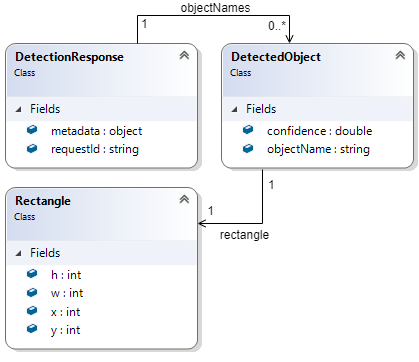
\includegraphics[width=0.6\textwidth]{images/dia_json.PNG}
	\caption[Klassendiagramm für Json-Umwandelung]{Klassendiagramm für die Umwandlung der Json-Datei in Objekte.}
	\label{dia:jsonClasses}
\end{figure}

Die gefundenen Objekte sollen im 3D-Raum mit einem Label gekennzeichnet werden. Dafür wird für jedes \textit{DetectedObject} die Methode \textit{Cast} von der Klasse \textit{PixelToWorld} aufgerufen. Zu diesem Zweck wird der \textit{Cast} Methode der Mittelpunkt der Bounding-Box als u,v Foto-Koordinaten für das \textit{DetectedObject} übergeben.

\begin{lstlisting}
public void HandleJsonResponse(System.String jsonResponse, SavedCameraState cpos)
{
	jsonResponse = jsonResponse.Replace("object", "objectName"); 
	//c# dosn't like "public string object"
	DetectionResponse det = new DetectionResponse();
	det = JsonUtility.FromJson<DetectionResponse>(jsonResponse);
	foreach (DetectedObject obj in det.objectNames)
	{
		Debug.Log(obj.objectName);
		int x = obj.rectangle.x + (obj.rectangle.w / 2);
		int y = obj.rectangle.y + (obj.rectangle.h / 2);
		PixelToWorld.instance.Cast(x, y, cpos, obj.objectName);
	}
}
\end{lstlisting}

%\begin{figure}[H]
%	\centering
%	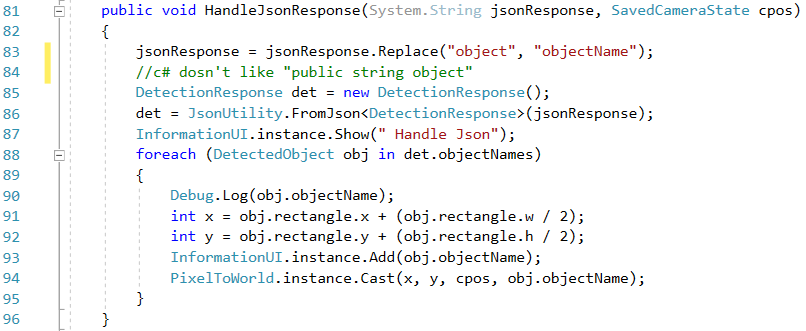
\includegraphics[width=1\textwidth]{images/code_handleJson.PNG}
%	\caption[Quellcode Umwandelung der Json Datei in Objekte]{Quellcode Umwandeln der Json Datei in Objekte.}
%	\label{code:handlejson}
%\end{figure}

\subsubsection{Von dem Foto zum 3D-Raum}

\begin{figure}[H]
	\centering
	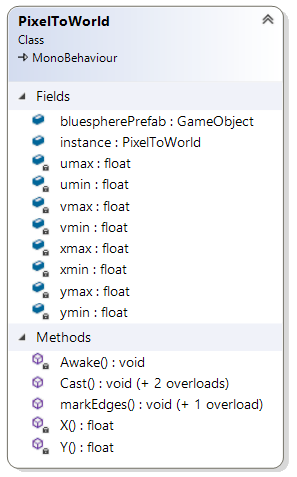
\includegraphics[width=0.45\textwidth]{images/dia_pixeltoworld.PNG}
	\caption[Klassendiagramm von \textit{PixelToWorld}]{Klassendiagramm von \textit{PixelToWorld}}
	\label{dia:pixeltoworld}
\end{figure}

Ein gefundenes Foto-Objekt soll in der 3D-Abbildung der realen Welt lokalisiert werden. Dafür nutzt die Methode \textit{Cast} sowohl die u,v Foto-Koordinaten des Objekts als auch einen \textit{SavedCameraState}. Der \textit{SavedCameraState} beschreibt die Position der Unity-Kamera zum Aufnahmezeitpunkt des Fotos.  \textit{SavedCameraState} beinhaltet zum einen die \textit{cameraToWorldMatrix} und zum anderen den Ursprung der Kamera.

Das Foto kann mit dem Display und somit mit der Clipping Plane der Unity-Kamera approximiert werden.
Die u,v Foto-Koordinaten werden in x,y,z Koordinaten des Camera Spaces umgewandelt. Die z-Achse verläuft durch den Ursprung der Kamera und folgt deren Blickrichtung. Punkte, welche sich auf der Clipping Plane befinden, sind 0.4 Einheiten von dem Ursprung der Kamera in Richtung der z-Achse entfernt. In dem Camera Space wird diese Entfernung mit z = -0.4 angegeben. 

Die x und y-Dimensionen beschreiben die Achsen, welche horizontal und vertikal zur Clipping Plane verlaufen. Mit dem festgelegten Wert z = -0.4, kann jeder Punkt auf der Clipping Plane mithilfe der Dimensionen x und y angegeben werden. Dazu gehören auch Punkte, welche außerhalb des View Frustums liegen.

Es wurden Werte für x und y ausprobiert, mit denen die Ränder des Fotos auf der Clipping Plane angegeben werden können. Dabei muss auf die unterschiedlichen Seitenverhältnisse des Fotos und des Displays geachtet werden. Darüber hinaus ist der Bildausschnitt des Displays kleiner. Daher liegen die Ränder des Fotos außerhalb des View Frustums. 

Mit den ausprobierten x und y-Werten ergeben sich Intervalle für die beiden Achsen x und y. Mithilfe einer  Kombination der beiden Intervalle, können alle möglichen Foto-Koordinaten auf die Clipping Plane abgebildet werden. Die Intervalle lauten: [-0.2949,0.2295] für x und [0.1546,-0.1507] für y. Durch die gewählten Intervallgrenzen wird die Position und Skalierung des Fotos in Relation zu dem Display berücksichtigt. Siehe Kapitel \ref{section:devpixeltoworld} für die Entwicklung der \textit{Cast} Methode und die Ermittlung der Intervallgrenzen.

Es werden zwei lineare Funktionen aufgestellt:
\begin{itemize}
	\item Die Funktion \textit{X} bildet das Intervall für u [0,1920] auf das Intervall für x [-0.2949,0.2295] ab.
	\item Die Funktion \textit{Y} bildet das Intervall für v [0,1080] auf das Intervall für y [0.1546,-0.1507] ab.
\end{itemize}

Die Funktionen sind folgendermaßen umgesetzt:

\begin{lstlisting}
//Picture u and v ranges
private float umin = 0;//left
private float umax = 1920;//right
private float vmin = 0;//up
private float vmax = 1080;//down
//Offset Vektor x and y ranges
private float xmin = -0.2949F;//left
private float xmax = 0.230F;//right
private float ymin = 0.1546F;//up
private float ymax = -0.1507F;//down

private float X(float u)
{
	float slope = ((xmax - xmin) / (umax - umin));
	float b = xmin - slope * umin;
	return slope * u + b;
}
private float Y(float v)
{
	float slope = ((ymax - ymin) / (vmax - vmin));
	float b = ymin - slope * vmin;
	return slope * v + b;
}
\end{lstlisting}

Mit den Funktionen wird eine Position im Camera Space für u,v berechnet. Diese Position wird, mithilfe der \textit{cameraToWorldMatrix} des \textit{SavedCameraState}, in eine Position \textit{p} des globalen Koordinatensystems umgewandelt. Auf diese Weise werden sowohl Position als auch Rotation der Kamera – und somit des Fotos – in der 3D-Szene berücksichtigt. %Siehe Abbildung \ref{code:castmethod}.

\begin{lstlisting}
public void Cast(float u, float v, SavedCameraState cpos,GameObject clippingPlaneMarker, string objectName, bool showClippingPlane, int material)
	{
	//scale v,v to x,y range
	Vector3 offset = new Vector3(X(u), Y(v), -0.4F);
	Vector3 p = cpos.cameratoWorldMatrix.MultiplyPoint(offset);
	Raycast.instance.StartCast(Raycast.instance.CreateRaycastParams(cpos.ctransform, p), objectName, material);
	if (showClippingPlane)// show point on clipping plane
	{
		GameObject sphere2 = Instantiate(clippingPlaneMarker, p, Quaternion.identity);
	}
}
\end{lstlisting}

%\begin{figure}[H]
%	\centering
%	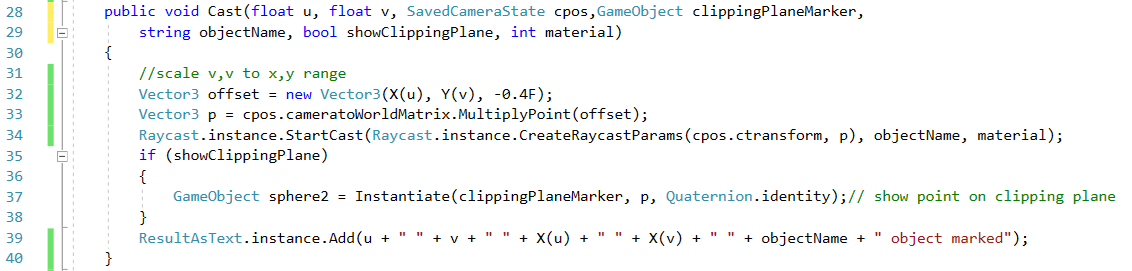
\includegraphics[width=1.2\textwidth]{images/code_cast_method.PNG}
%	\caption[Quellcode der Cast Methode]{Quellcode der Cast Methode}
%	\label{code:castmethod}
%\end{figure}
\subsubsection{Raycast}

\begin{figure}[H]
	\centering
	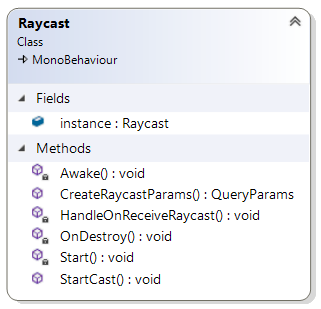
\includegraphics[width=0.45\textwidth]{images/dia_raycast.PNG}
	\caption[Klassendiagramm von Raycast]{Klassendiagramm von Raycast}
	\label{dia:raycast}
\end{figure}

Als Nächstes wird ein Raycast durch den Ursprung der Kamera und die Position \textit{p} gesendet. \textit{MLRaycast} wird genutzt, um einen Schnittpunkt mit der Rekonstruktion der Welt von Lumin OS zu bestimmen. Die Stelle, welche von dem Raycast getroffen wird, beschreibt die Position des \textit{DetectedObject} im 3D-Raum.

Für den \textit{MLRaycast} werden zwei Parameter benötigt:
\begin{itemize}
	\item Ein \textit{QueryParams} Objekt, das Ursprung und Richtung für den Raycast beinhaltet.
	\begin{itemize}
		\item Ursprung: Kamera-Ursprung aus \textit{SavedCameraState}
		\item Richtung: Richtungsvektor von dem Kamera-Ursprung zu der Position \textit{p}
	\end{itemize}
	\item Eine Methode die aufgerufen wird, wenn der Raycast fertig ist. 
	\begin{itemize}
		\item Callback Methode: \textit{HandleOnRecieveRaycast}
	\end{itemize}
\end{itemize}

%Siehe Abbildung \ref{code:raycastparams}.

%\begin{figure}[H]
%	\centering
%	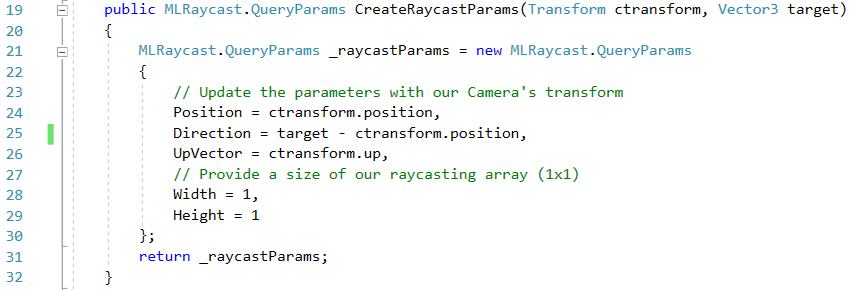
\includegraphics[width=1\textwidth]{images/code_raycastparams.PNG}
%	\caption[Quellcode Erzeugung der Raycast Parameter]{Quellcode Erzeugung der Raycast Parameter}
%	\label{code:raycastparams}
%\end{figure}

\begin{lstlisting}
public MLRaycast.QueryParams CreateRaycastParams(Transform ctransform, Vector3 target)
{
	MLRaycast.QueryParams _raycastParams = new MLRaycast.QueryParams
	{
		// Update the parameters with our Camera's transform
		Position = ctransform.position,
		Direction = target - ctransform.position,
		UpVector = ctransform.up,
		// Provide a size of our raycasting array (1x1)
		Width = 1,
		Height = 1
	};
	return _raycastParams;
}
\end{lstlisting}
Wenn der Raycast fertig ist, wird die Methode \textit{HandleOnRecieveRaycast} aufgerufen. Der Parameter \textit{point} beinhaltet dabei die von dem Raycast getroffene Stelle der AR-Umgebung. Diese wird an die Methode \textit{CreateMarker} von der Klasse \textit{LabelCreater} weitergegeben.

\subsubsection{LabelCreater}

%\begin{figure}
%	\centering
%	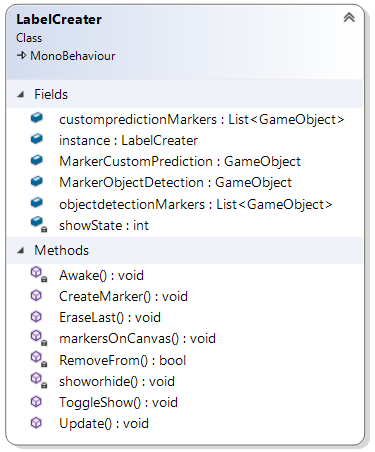
\includegraphics[width=0.5\textwidth]{images/dia_labelcreater.PNG}
%	\caption[]{Markierungen in der Welt}
%	\label{dia:labelcreater}
%\end{figure}

\textit{CreateMarker} erhält den Punkt \textit{point}, der getroffen wurde und die Bezeichnung für das \textit{DetectedObject}. An der Position von \textit{point} wird ein Prefab GameObject instanziiert, das als Label für das \textit{DetectedObject} in der 3D-Umgebung dient. Das Prefab besteht aus einer Sphäre und einem Schriftzug. Dem neu instanziierten GameObject wird die Bezeichnung des \textit{DetectedObject} als Schriftzug zugewiesen. Siehe Abbildung \ref{image:labels}.

\begin{figure}[H]
	\centering
	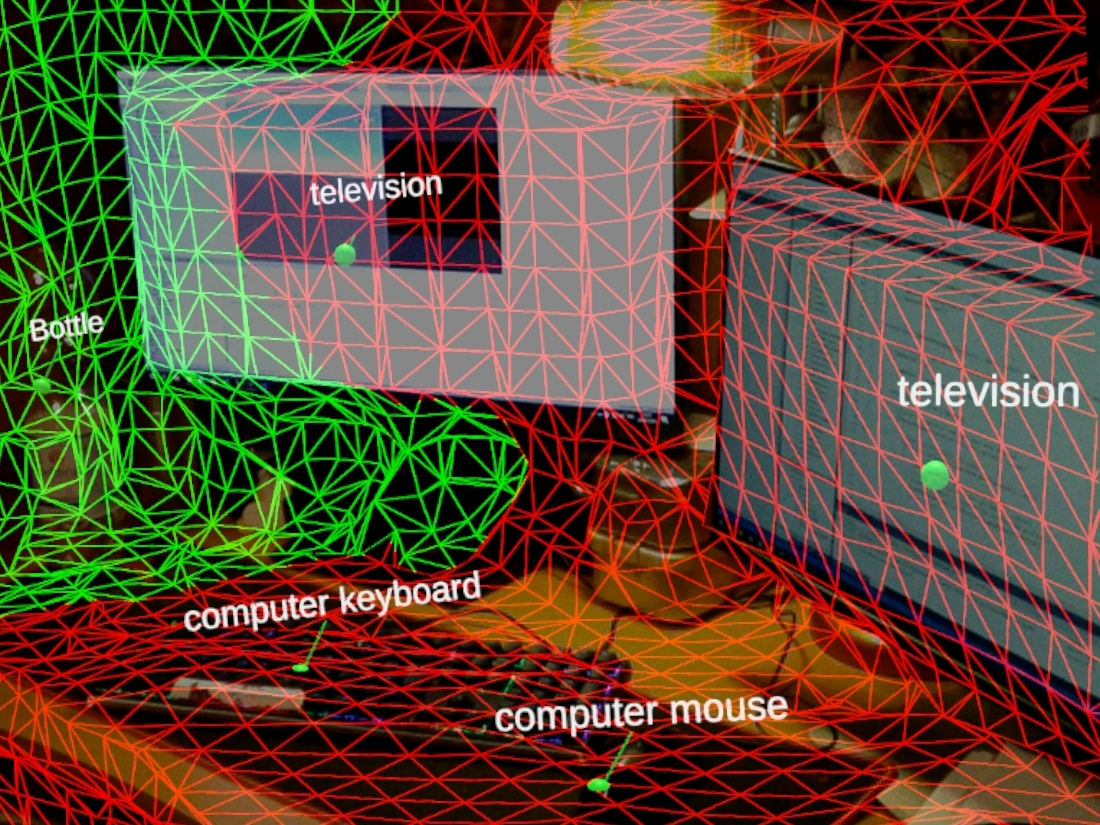
\includegraphics[width=0.8\textwidth]{images/ML_20201004_19.10.05_2.jpg}
	\caption[Labels in der Szene]{Labels in der Szene}
	\label{image:labels}
\end{figure}

%todo read this over
Bevor ein neues Label erzeugt werden kann, muss überprüft werden, ob das Objekt, welches dadurch annotiert werden soll, bereits ein Label hat.

Zu diesem Zweck werden alle bereits existierenden Labels durchgegangen. Dabei wird nach Labels gesucht, die in der Nähe des zukünftigen Labels liegen und denselben Schriftzug aufweisen. Bei Auffinden eines solchen Labels wird davon ausgegangen, dass es sich auf dasselbe Objekt bezieht wie das zukünftige Label. In diesem Falle wird kein neues Label erzeugt, sondern das Alte modifiziert. Diese Modifikation ist in der Methode \textit{UpdateLocation} des \textit{MarkerBehaviors} implementiert, welches jedes Label besitzt. Der Methode \textit{UpdateLocation} wird die 3D-Position übergeben, an welcher ursprünglich das neue Label erzeugt werden sollte.

\textit{MarkerBehavior} speichert alle 3D-Positionen in einer Liste ab, die jemals für das dazugehörige Label angegeben wurden. Dazu zählen sowohl die Position an welcher das Label initialisiert wurde, als auch alle Positionen, die durch \textit{UpdateLocation} übergeben wurden. Eine neu übergebene 3D-Position wird durch eine kleine Sphäre markiert. Das Label wird in den Mittelpunkt aller gespeicherten Positionen gesetzt.

Als Resultat werden alle Positionen, an welchen das Objekt in der Szene lokalisiert wurde, jeweils mit einer kleinen Sphäre markiert. Das Label befindet sich im Mittelpunkt aller Positionen. Siehe Abbildungen \ref{image:multi1} und \ref{image:multi2}.

%sondern das  ein Label nahe eines anderen Labels erzeugt werden soll, das denselben Schriftzug hat, wird davon ausgegangen, das ein Objekt der realen Welt erneut erkannt wurde. Daher wird kein neues Label erstellt, sondern das alte Label modifiziert. Die Positionen, an denen das Objekt in der Szene lokalisiert wurde, werden jeweils mit kleineren Sphäre markiert und das Label wird in den Mittelpunkt der kleinen Sphären gesetzt. So wird die Position des Objektes genauer, wenn es häufiger erkannt wurde. Siehe Abbildungen \ref{image:multi1} und \ref{image:multi2}.

\begin{figure}[H]
	\centering
	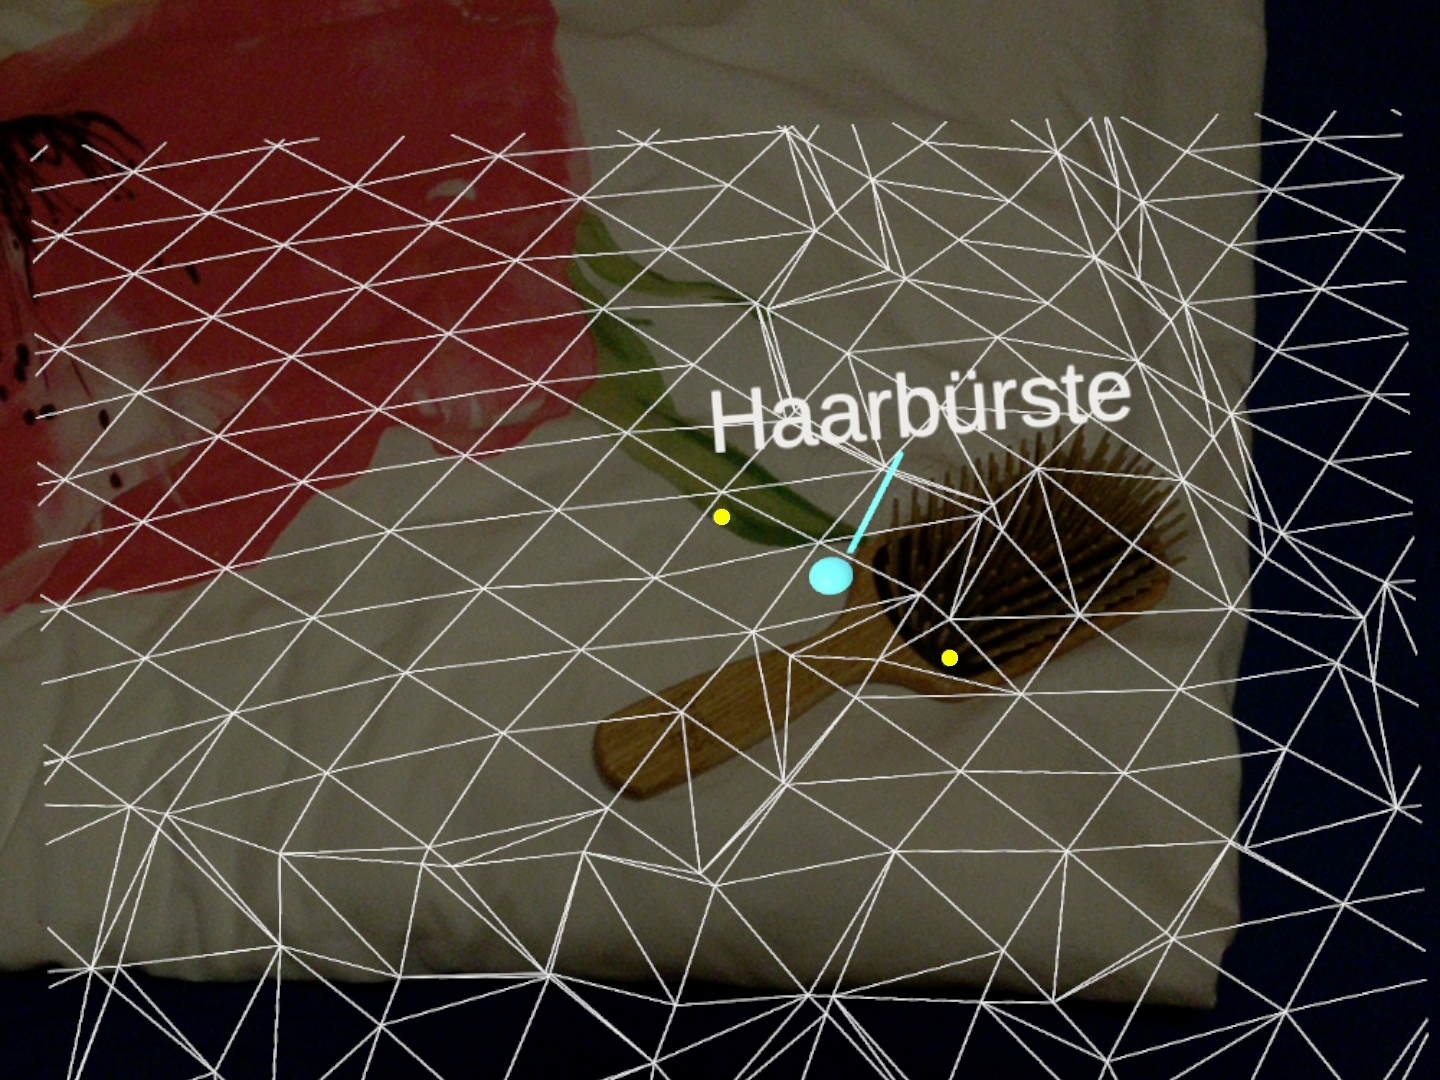
\includegraphics[width=0.7\textwidth]{images/ML_multi1.jpg}
	\caption[Haarbürste zwei mal erkannt]{Haarbürste zweimal erkannt.}
	\label{image:multi1}
\end{figure}


\begin{figure}[H]
	\centering
	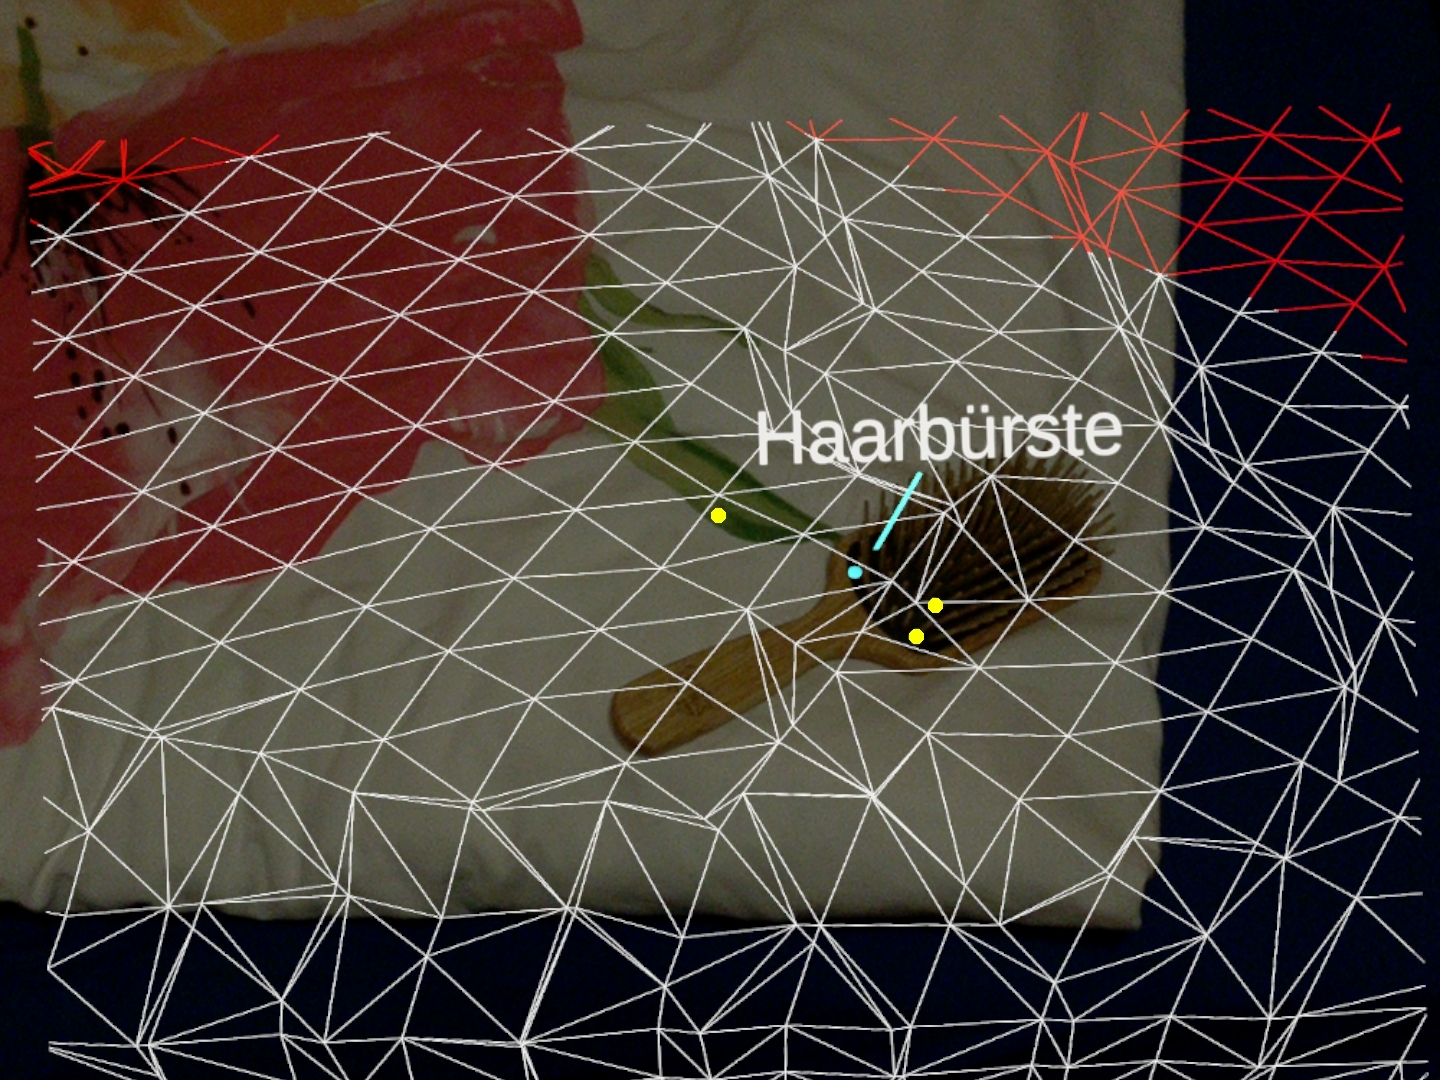
\includegraphics[width=0.7\textwidth]{images/ML_multi2.jpg}
	\caption[Haarbürste drei mal erkannt]{Haarbürste dreimal erkannt.}
	\label{image:multi2}
\end{figure}


Bei jedem Frame der Applikation werden alle Labels zur Kamera hingedreht, sodass eine rechtwinklige Ausrichtung zur Kamera erfolgt. Dieses Verhalten ist in \textit{MarkerBehavior} implementiert. 

\begin{lstlisting}
public void Update()
{
	mainMarker.transform.LookAt(Camera.main.transform.position);
}
\end{lstlisting}

Auf diese Weise werden die Labels der Kamera nachgeführt. Solange ein Label in dem View Frustum liegt, kann der Nutzer es lesen. Siehe Anhang \ref{appendix:blickwinkel}.

\subsubsection{Azure Custom Vision}

Neben 'Azure Object Detection' wird auch der Service 'Azure Custom Vision' zur Bildanalyse verwendet. Dieser Service bietet ein Object Detection Modell an, welches mithilfe einer Webseite trainiert wird. Als 'Iteration' wird ein trainiertes KI-Modell bezeichnet. Dieses kann zur Objekterkennung verwendet werden. Die Anfragen an eine Iteration geschieht in der Klasse \textit{AzureCustomPrediction}. Ähnlich wie bei \textit{AzureObjectDetection} wird ein Webrequest erstellt. Dieser beinhaltet einen Authentifizierungs-Schlüssel und ein Foto. Die Anfragen an die beiden Services werden parallel in unterschiedlichen Threads erstellt und bearbeitet.

In der Antwort wird eine Json-Datei zurückgeschickt, welche die gefundenen Objekte angibt. Da die Json-Datei ein etwas anderes Format als das Analyseresultat von Azure Object Detection hat, verfügt \textit{AzureCustomVision} über eine eigene \textit{HandleJsonResponse} Methode. Dabei gibt Azure Custom Vision für jedes \textit{DetectedObject} eine Probability an. Diese sagt aus, wie groß das Vertrauen des Modells darin ist, dass das Objekt korrekt erkannt wurde. Mithilfe eines definierten Schwellenwerts wird entschieden, wie hoch die Probability mindestens sein muss, um das Objekt zu akzeptieren und in der Szene zu markieren.

Für jedes akzeptierte Objekt wird die Methode \textit{Cast} von \textit{PixelToWorld} aufgerufen. Diese Methode behandelt alle Objekte gleich,  unabhängig davon, von welchem Object Detection Service sie erkannt wurden - entweder von Azure Custom Vision oder von Azure Object Detection. Die Position des Objektes wird in der Szene mithilfe von \textit{Cast} und einem Raycast lokalisiert. Anschließend erzeugt \textit{LabelCreater} ein Label an der entsprechenden Position. 

Labels für Objekte von Azure Custom Vision unterscheiden sich lediglich durch eine unterschiedliche Farbgebung von Labels, welche durch Azure Objekt Detection erzeugt werden. 

\paragraph{Iterationen von Azure Custom Vision}

Das Custom Vision Modell wird auf drei unterschiedliche Objekte trainiert: eine Farbtube, eine blaue Dose und eine Haarbürste. Dabei werden sechs Iterationen erstellt. 

\paragraph{Iteration 1}

Die Iteration 1 ist darauf trainiert, eine Farbtube zu erkennen. Bei der Nutzung dieser Iteration tritt das Problem vieler fehlerhafter Objekterkennungen auf. Es werden Acrylfarben an Stellen erkannt, an denen es keine gibt. Siehe Abbildung \ref{image:customVisionPaint}. 

Die Evaluierung des Modelles lautet: 66.7\% Precision, 66.7\% Recall, 89.7\% mean Average Precision.
In der Testphase kann das Modell 66,7\% der Nivea-Dosen auf den Bildern erkennen (Recall) und 66,7\% der Objekte die als Nivea-Dosen markiert werden, sind tatsächlich Nivea-Dosen (Precision).

\begin{figure}[H]
	\centering
	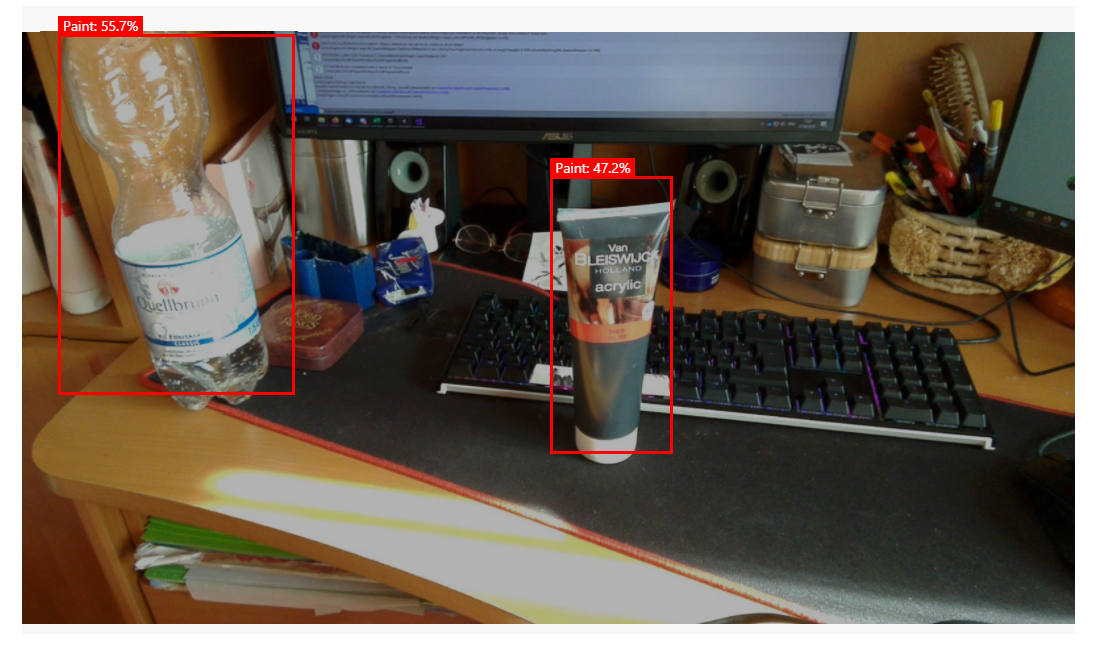
\includegraphics[width=0.8\textwidth]{images/customVisionPaint.PNG}
	\caption[Iteration 1 Analysebeispiel]{Iteration 1 Analysebeispiel. Eine Wasserflasche und eine Farbtube werden beide als Farbtuben erkannt. Die Wasserflasche wird mit einer Probability von 55.7 Prozent markiert, während die tatsächliche Farbtube eine Probability von 47.5 Prozent hat.}
	\label{image:customVisionPaint}
\end{figure}

\paragraph{Iteration 2}

Die Iteration 2 wird darauf trainiert, eine blaue Nivea-Dose zu erkennen. Form und Farbe der Dose sind sehr simpel. Dennoch ist auch dieser Gegenstand nicht leicht zu erkennen. 

Die Evaluierung des Modells lautet: 80\% Precision, 100\% Recall, 100\% mean Average Precicion.
Das bedeutet: In der Testphase kann das Modell alle auf den Bildern erhaltenen Nivea-Dosen erkennen (100\% Recall). Es markiert jedoch auch Objekte als Dosen, die keine Dosen sind (80\% Precision).

Auch bei der Nutzung der Iteration außerhalb der Testphase werden viele Gegenstände fälschlicherweise als Nivea-Dosen erkannt (false positives). 


\paragraph{Iteration 3}

Mit der Iteration 3 wird eine Verbesserung von Iteration 2 beabsichtigt. Für diesen Zweck wird die Menge an Trainingsdaten um 10 zusätzliche Fotos erweitert. Die Datenmenge steigt damit von ursprünglich 18 auf 28 Fotos. In den Trainingsdaten wird die Dose auf unterschiedlichen Hintergründen abgebildet, welche sich durch Farbe und Muster unterscheiden. 

Die Evaluierung des Modells lautet: 75\% Precision, 100\% Recall, 100\% mean Average Precicion. Auch diese Iteration markiert in der Testphase häufig Objekte fälschlicherweise als Dosen (75\% Precision). Bei der Verwendung außerhalb der Testphase werden ebenfalls Objekte fälschlicherweise als Dosen markiert. Die beabsichtigte Verbesserung ist damit nicht gelungen.

\paragraph{Iteration 4}

Mit der Iteration 4 wird ein weiterer Verbesserungsversuch durchgeführt. Zu diesem Zweck werden solche Trainingsfotos aus der Datenmenge entfernt, welche die Dose aus einem seitlichen Blickwinkel zeigen. Die Dose soll nur erkannt werden, wenn sie auf dem Foto von oben zu sehen ist. Erwartet wird, dass während der Nutzung der Iteration weniger Gegenstände fälschlicherweise als Nivea-Dose erkannt werden.

In der Testphase wird diese Erwartung erfüllt: Precision und Recall der Nivea-Dose steigen auf 100 Prozent. Das Modell kann in dem Test alle Nivea-Dosen fehlerfrei erkennen. Bei der Verwendung des Modells außerhalb der Testphase zeigt sich allerdings, ein anderes Ergebnis: Häufig werden Objekte fälschlicherweise als Nivea-Dose markiert. Dies liegt die Vermutung nahe, dass das Objekt 'Nivea Dose' grundsätzlich problematisch für die Object Detection ist. Dies könnte an der Homogenität des Objektes liegen. 

Diese Vermutung wird anhand eines Objektes mit markanterer Struktur überprüft. Die Wahl fällt auf eine Holzhaarbürste. Wird dieses Objekt - mit den Borsten nach oben zeigend - fotografiert, weist es ein markantes Muster auf. Aufgrund von ihres komplexeren Aussehens ist davon ausgegangen, dass die Bürste leichter von anderen Gegenständen zu unterscheiden ist, als dies bei der Dose der Fall war. Es werden 16 Trainingsbilder für die Erkennung der Bürste aufgenommen. Wie beschrieben, wird darauf geachtet, dass die Borsten nach oben zeigen. Siehe Anhang \ref{appendix:it4train}.

Die Evaluierung der Haarbürsten-Objekterkennung lautet: 100\% Precision, 100\% Recall, 100\% Average Precision. Das bedeutet: In der Trainingsphase werden alle Haarbürsten fehlerfrei erkannt. 

Bei Verwendung der Iteration 4 außerhalb der Trainingsphase zeigt sich, dass die Haarbürste tatsächlich leichter von anderen Objekten unterschieden werden kann, als dies bei der Dose der Fall war.

Es lässt sich beobachten, dass Objekte, welche mit einer Probability von 80 Prozent als Haarbürste markiert werden, tatsächlich Haarbürsten sind. Durch das Setzen dieses Schwellenwertes können korrekte Objekterkennungen von false postives unterschieden werden. Siehe Abbildung \ref{img:it4}.

\begin{figure}[H]
	\centering
	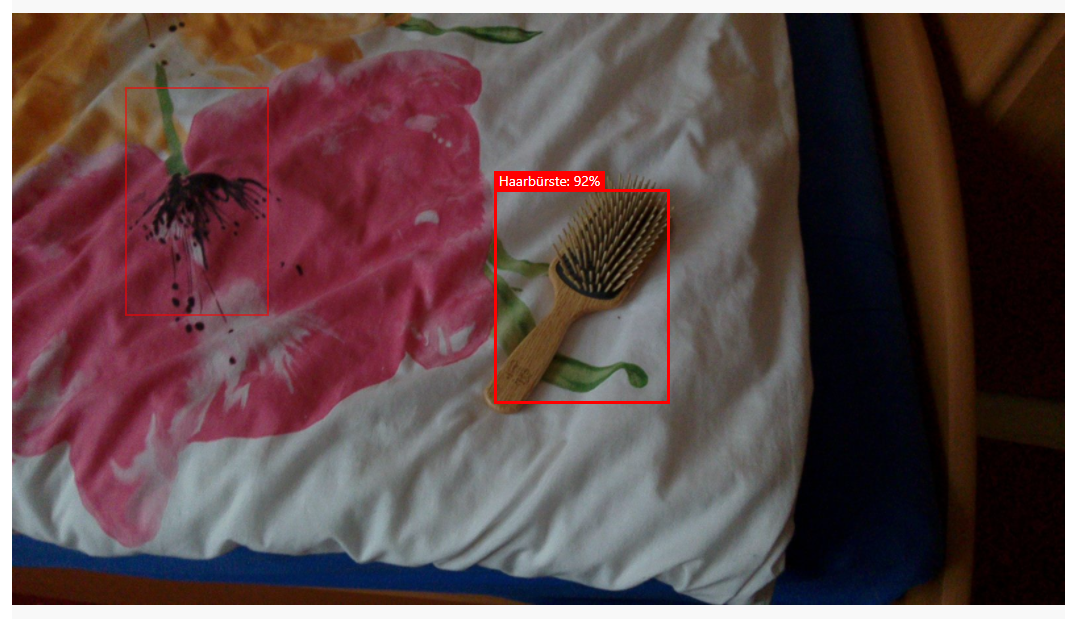
\includegraphics[width=0.8\textwidth]{images/it4notpretty.png}
	\caption[Iteration 4 Analysebeispiel]{Iteration 4 Analysebeispiel. Die tatsächliche Haarbürste wurde mit einer Probability von 92 Prozent erkannt. Eine Blume auf einer Decke wurde zu 71,3 Prozent als Haarbürste erkannt.}
	\label{img:it4}
\end{figure}

Wenn die Haarbürste in dem Foto relativ wenig Platz einnimmt, wird sie mit einer geringeren Probability erkannt. Dadurch ist es nicht mehr möglich, die Bürste mithilfe eines Schwellenwertes von anderen Objekten zu unterscheiden.

\begin{figure}[H]
	\centering
	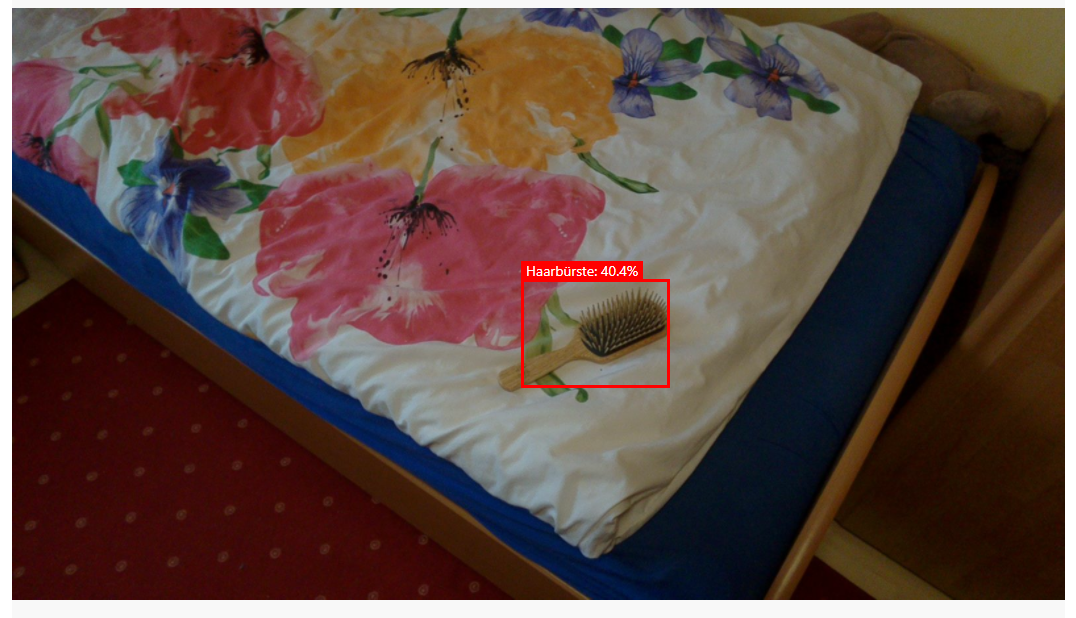
\includegraphics[width=0.8\textwidth]{images/it4notpretty2.png}
	\caption[Iteration 4 zweites Analysebeispiel]{Iteration 4 Analysebeispiel. Die tatsächliche Haarbürste wurde mit einer Probability von 40,4 Prozent erkannt.}
	\label{img:it4}
\end{figure}
\paragraph{Iteration 5}

Iteration 5 ist eine Variation von Iteration 4. In dem Training wird die Objekterkennung der Nivea-Dose entfernt. Diese Iteration ist nur noch darauf trainiert, das Objekt Haarbürste zu erkennen. Die Trainingsbilder für das Objekt Haarbürste bleiben unverändert. Die Evaluierung des Modells lautet: 100\% Precision, 100\% Recall, 100\% mean Average Precicion.

Die Genauigkeit der Haarbürsten-Erkennung bleibt unverändert.

\paragraph{Iteration 6}

In der Iteration 6 wird die Erkennung der Haarbürste verbessert. Ziel ist es, auch kleine Abbildungen der Haarbürste fehlerfrei zu erkennen. Den Empfehlungen von Azure folgend, wird die Menge an Trainingsbildern auf 51 erhöht. Weiterhin zeigt die Haarbürste in allen Bildern mit den Borsten nach oben. Auf den neuen Trainingsbildern ist die Haarbürste teilweise recht klein zu sehen. Siehe Anhang \ref{appendix:it4train}. Der Iteration 6 wird eine Stunde Zeit gelassen, um das Training durchzuführen. Der Trainingsprozess der vorherigen Iterationen 5 und 4 dauerte lediglich ca. 10 Minuten.

Die Evaluierung von Iteration 6 in der Testphase lautet: 100\% Precision, 100\% Recall, 100\% mean Average Precision. Das auch diesmal die Testphase fehlerfrei durchlaufen wird. 

Bei der Verwendung der Iteration außerhalb der Testphase können diesmal auch Haarbürsten erkannt werden, die in einem Foto klein abgebildet sind. Siehe Abbildung \ref{img:it6}. 

\begin{figure}[H]
	\centering
	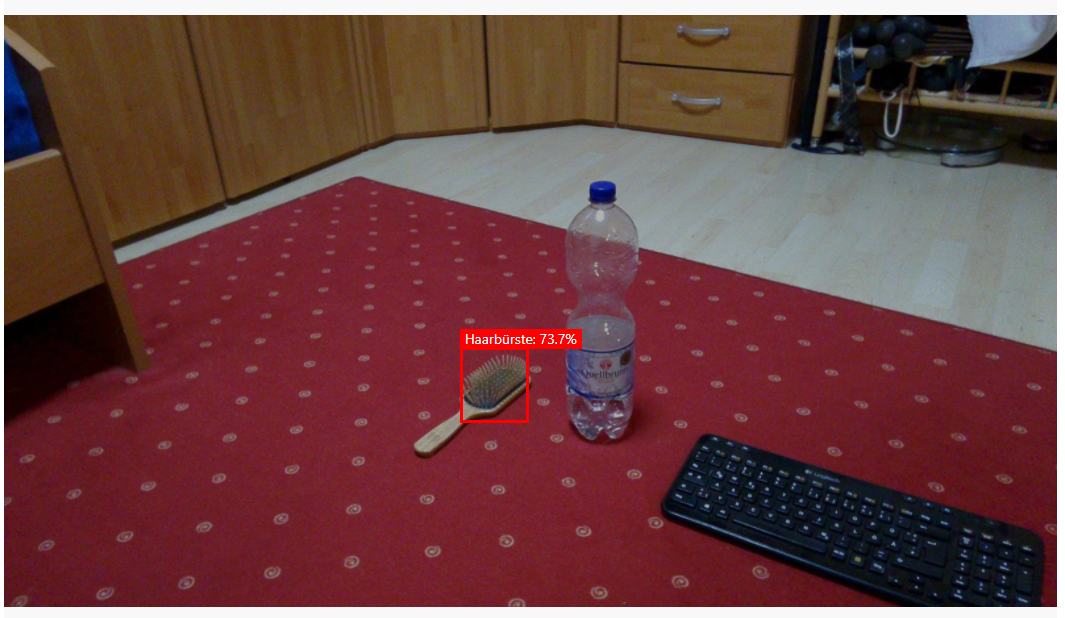
\includegraphics[width=0.75\textwidth]{images/it6pretty.png}
	\caption[Iteration 6 Analysebeispiel]{Iteration 6 Analysebeispiel. Die Haarbürste wurde mit einer Probability von 73,7 Prozent erkannt.}
	\label{img:it6}
\end{figure}

Somit ist das Ziel der Iteration 6 erfüllt. In den Bildern, die von Iteration 6 analysiert werden, sind alle Objekte die mit einer Probability von über 50 Prozent als Haarbürste markiert werden, tatsächlich Haarbürsten. Korrekte Objekterkennungen lassen sich gut von false positives unterscheiden. 


\subsection{Entwicklung der Foto-Repräsentation}
\label{section:devpixeltoworld}

In diesem Abschnitt wird die Entwicklung der \textit{Cast} Methode beschrieben.
%Diese Methode implementiert die Foto-Repräsentation. Sie transformiert u,v Foto-Koordinaten in eine Position auf der Clipping Plane der Unity-Kamera. Diese Funktionalität wird für die Lokalisierung von Objekten in dem 3D-Raum verwendet.

Ziel dieser Methode ist das Setzen einer Markierung in der 3D-Szene, basierend auf gegebenen Foto-Koordinaten. Das Foto beinhaltet keine Information über die Entfernung eines Objektes zur Kamera. Um die Entfernung zu ermitteln, ist ein Raycast erforderlich. Mit einer Repräsentation des Fotos in der 3D-Szene ist es möglich, diesen Raycast durchzuführen. Dazu muss das Foto nicht tatsächlich in dem 3D-Raum vorhanden sein. Es wird lediglich mit Koordinaten gearbeitet. Es muss die Möglichkeit existieren, die Foto-Position eines Objektes in eine Position der 3D-Szene umzuwandeln. Letztere muss das Verhältnis der Foto-Position zu der Umgebung widerspiegeln. Wenn diese Funktionalität erfüllt ist, kann die Position der 3D-Szene dafür verwendet werden, einen Raycast auf die Umgebung durchzuführen und somit die korrekte Position für den Gegenstand zu finden.

Die Position des Fotos hängt mit der Unity-Kamera zusammen. Daher kann das Foto durch den Camera Space simuliert werden. Als Erstes wird probiert ein Sphären-Objekt an eine gezielte Koordinate des Camera Spaces zu setzten. Unter den Voraussetzungen, dass die Kamera sowohl am Ursprung des globalen Koordinatensystems liegt als auch eine neutrale Rotation aufweist, stimmt der Camera Space mit dem globalen Koordinatensystem überein. Die Sphäre wird in der Szene per Hand bewegt, um markante Koordinaten des Camera Spaces abzulesen. Siehe Abbildung \ref{illustration:speretest}.

\begin{figure}[H]
	\centering
	\includegraphics[width=0.5\textwidth]{images/sphärenTestwhite.jpg}
	\caption[Ränder der Near Clipping Plane in Unity finden]{Die weiße Sphäre liegt auf dem linken Rand der Clipping Plane.}
	\label{illustration:speretest}
\end{figure}

Dabei werden folgende Camera Space Koordinaten gefunden:
\begin{itemize}
	\item Near Clipping Plane bei z = -0.37
	\item linker Rand bei x = -0.153
	\item rechter Rand bei x = 0.153
	\item oberer Rand bei y = 0.1147
	\item unterer Rand bei y = -0.1147
\end{itemize}

Die x und y-Koordinaten hängen von den u,v Koordinaten des Fotos ab. Daher werden lineare Funktionen aufgestellt, um u,v auf x,y abzubilden. Diese Abbildungen dienen als Repräsentation des Fotos im 3D-Raum. Sie berücksichtigen sowohl die Postion als auch die Skalierung des Fotos im Verhältnis zu der Unity-Kamera.

Diese Version der Foto-Repräsentation wird getestet. Geprüft wird, wie gut die Lokaliserung von \textit{DetectedObjects} in der AR-Umgebung gelingt. Es zeigt sind, dass die entstehenden Markierungen zwar in dem View Frustum liegen, jedoch nicht die korrekten Positionen der \textit{DetectedObjects} angeben.

Zur Problemanalyse wird ein UI-Objekt erstellt, welches während der Laufzeit die aufgenommenen Fotos anzeigt. Mithilfe des UI-Objektes werden die Fotos mit dem Sichtfeld des Displays verglichen. Dabei ist zu beobachten, dass Foto und Display ein unterschiedliches Seitenverhältnis haben. Darüber hinaus zeigt das Display einen kleinen Bildausschnitt an.

Es gibt zwei Möglichkeiten, die Unterschiede zwischen Foto und Display auszugleichen: Entweder wird das Foto auf das Display zugeschnitten oder das gesamte Foto wird verwendet. Letztere Möglichkeit würde dazu führen, dass auch Objekte erkannt werden, welche außerhalb des Sichtfeldes liegen. Dies würde zu einem inkonsistenten Feedback für den Nutzer führen, da manche Labels außerhalb seines Sichtfeldes entstünden. Um diesen Nachteil zu umgehen, wird die Entscheidung getroffen, das Foto auf das Display zuzuschneiden.

Das Zuschneiden wird realisiert, indem die Intervalle für u und v der Abbildungsfunktionen stärker eingegrenzt werden. Ignoriert werden alle Objekte, die außerhalb der Intervalle liegen. Um die neuen Intervallgrenzen zu bestimmen, wird dem Fotoanzeige-UI-Element ein Gitter-Element hinzugefügt. Mit dem Gitter kann die u,v Position von beliebigen Stellen des Fotos abgelesen werden. Durch Fotoaufnahmen und Vergleiche mit dem Sichtfeld des Displays wird abgelesen, bei welcher u,v Position des Fotos die Ecken des Displays zu finden sind. Die Intervalle werden dementsprechend eingegrenzt. 

Mit den durchgeführten Veränderungen der Intervallgrenzen können \textit{DetectedObjects} zwar prinzipiell korrekt in der Umgebung lokalisiert werden. Als problematisch erweisen sich allerdings solche Objekte, die nur teilweise im Sichtfeld des Nutzers liegen. Der Mittelpunkt dieser Objekte liegt nämlich knapp außerhalb der Intervalle. Daher werden die Objekte ignoriert, obwohl der Nutzer von einer Markierung ausgeht. 

Die Zugschneidung des Fotos führt somit aus der Sicht des Nutzers zu einem inkonsistenten Verhalten, bezüglich der Objekterkennung. Darüber hinaus dauert es bei dem Verfahren mit den zugeschnittenen Fotos insgesamt länger einen Raum mit Labels zu versehen, da bei jeder Bildanalyse Daten verworfen werden. 

Die Zugschneidung der Fotos bringt daher zu viele Nachteile mit sich. Daher wird darauf verzichtet. Stattdessen werden die unbeschnittenen Fotos verwendet.

Um den Zuschnitt rückgängig zu machen, werden die Intervalle für u und v wieder auf die ursprünglichen Werte – [0,1920] und [0,1080] –  gesetzt. Folgerichtig müssen auch die Intervalle für x und y vergrößert werden. Um die x und y-Intervallgrenzen zu bestimmen, wird das Fotoanzeige-UI-Element parallel zu der Clipping Plane positioniert. Das Element folgt den Bewegungen der Kamera und ist möglichst nah an der Near Clipping Plane platziert. Siehe Abbildungen \ref{illustration:canvasinsourface} und \ref{illustration:canvasinsourfacetodown}.

\begin{figure}[H]
	\centering
	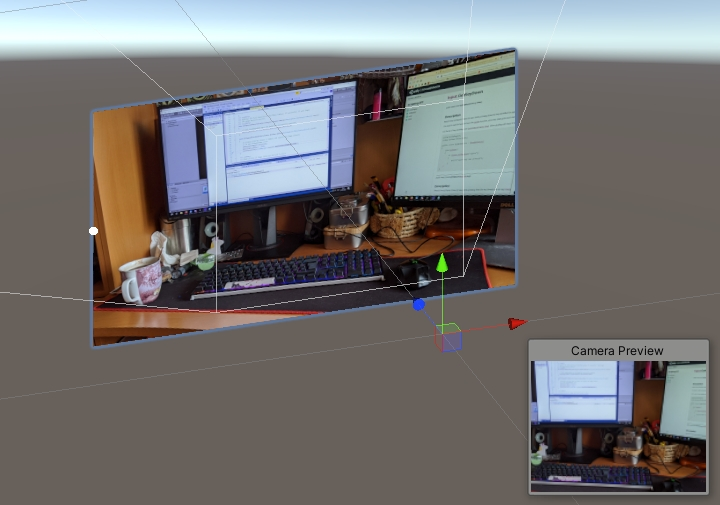
\includegraphics[width=0.7\textwidth]{images/canvasinyourface2.jpg}
	\caption[Ränder des Foto-Anzeige-Elements finden]{Bei der Anzeige füllt das aufgenommene Foto das gesamte Display aus. Die weiße Sphäre befindet sich auf dem linken Rand des Foto-Anzeige-Elementes.}
	\label{illustration:canvasinsourface}
\end{figure}

\begin{figure}[H]
	\centering
	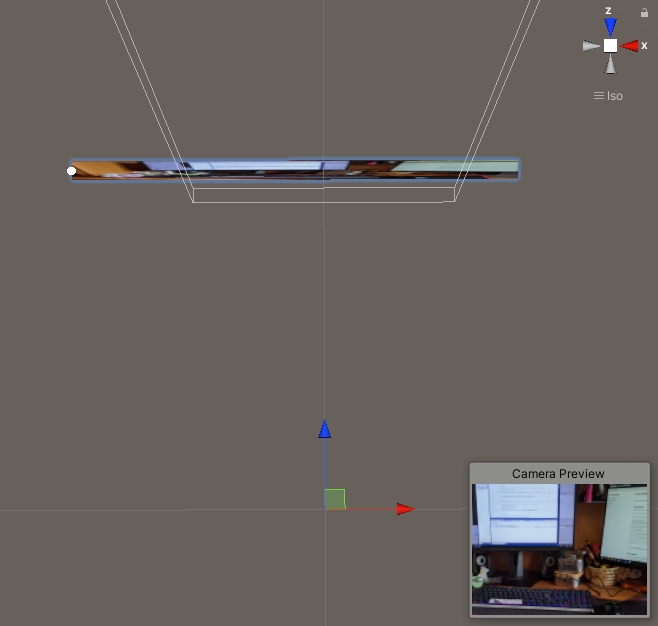
\includegraphics[width=0.58\textwidth]{images/canvasinyourfaceTopDown2.jpg}
	\caption[Tiefe des Foto-Anzeige-Elements finden]{Die weiße Sphäre befindet sich nicht mehr in dem View Frustum und das Foto-Anzeige-Element befindet sich ein wenig hinter der Near Clipping Plane.}
	\label{illustration:canvasinsourfacetodown}
\end{figure}

Das Display der Magic Leap Brille zeigt sogar solide Objekte leicht transparent an. Diese Eigenart des AR-Displays wird genutzt, um aufgenommene Fotos mit der realen Welt zu vergleichen. Durch Ausprobieren wird das UI-Element so skaliert und verschoben, dass das angezeigte Foto mit der realen Welt so weit wie möglich übereinstimmt. Das bedeutet, dass der Nutzer möglichst wenig Unterschiede zwischen dem angezeigten Foto und der durchschimmernden realen Welt sieht.

Die Ränder des skalierten UI-Elementes werden genutzt, um die Intervalle für x und y zu bestimmen.
\begin{itemize}
	\item für x: [-0.2949, 0.2295]
	\item für y: [0.1546, -0.1507]
	\item Zusätzlich wurde z = -0.4 gesetzt. Das UI Element musste ein wenig weiter von der Near Clipping Plane entfernt sein, um angezeigt zu werden.
\end{itemize}

Mit diesen Intervallen können \textit{DetectedObjects} gut lokalisiert werden. Zudem werden keine Objekte weggelassen, von denen Markierung der Nutzer ausgeht.

\newpage
\section{Auswertung}

In diesem Kapitel geht es um die Evaluierung und Auswertung der vorgestellten Anwendung.

\subsection{Laufzeitanalyse}

\subsubsection{Netzwerk}

Die genutzte Netzwerkverbindung hat eine Download-Geschwindigkeit von 180 Mbps und ein Upload-Geschwindigkeit von 18 Mbps. Mit einer Bildauflösung von 1090x1820 Pixeln, haben die Foto ein Größe von 5 Mb. 

Getestet wird der Netzwerk-Delay zwischen den REST-APIs der Objekterkennungsservices und der AR-Brille. Zu diesem Zweck wird eine HTTP-Anfrage mit einem inkorrekten Authentifizierungsschlüssel an die Services geschickt. In dem Body der Anfrage wird ein Bild mitgeschickt. Es ergibt sich Folgendes: Die Analyse wird abgelehnt, da die Authentifizierung fehlschlägt. Daraufhin wird umgehend eine Response Nachricht zurückgeschickt. Die Länge des Round-Trip-Times wird mit dem Netzwerk-Delay gleichgesetzt, da keine Analyse stattfindet. Die durchschnittliche Round-Trip-Time beträgt 0,18 Sekunden (minimal 0,13 Sekunden und maximal 0,28 Sekunden). Dieser Durchschnitt ergibt sich aus der Auswertung von 14 Tests.

\subsubsection{Objekterkennung}
Die Laufzeit der automatischen Objekterkennung für AR wird aufgezeichnet. Die Erkennung beginnt mit der Fotoaufnahme und endet mit der Erzeugung der Labels.
Siehe Abbildung \ref{img:laufzeit}

\begin{figure}[H]
	\centering
	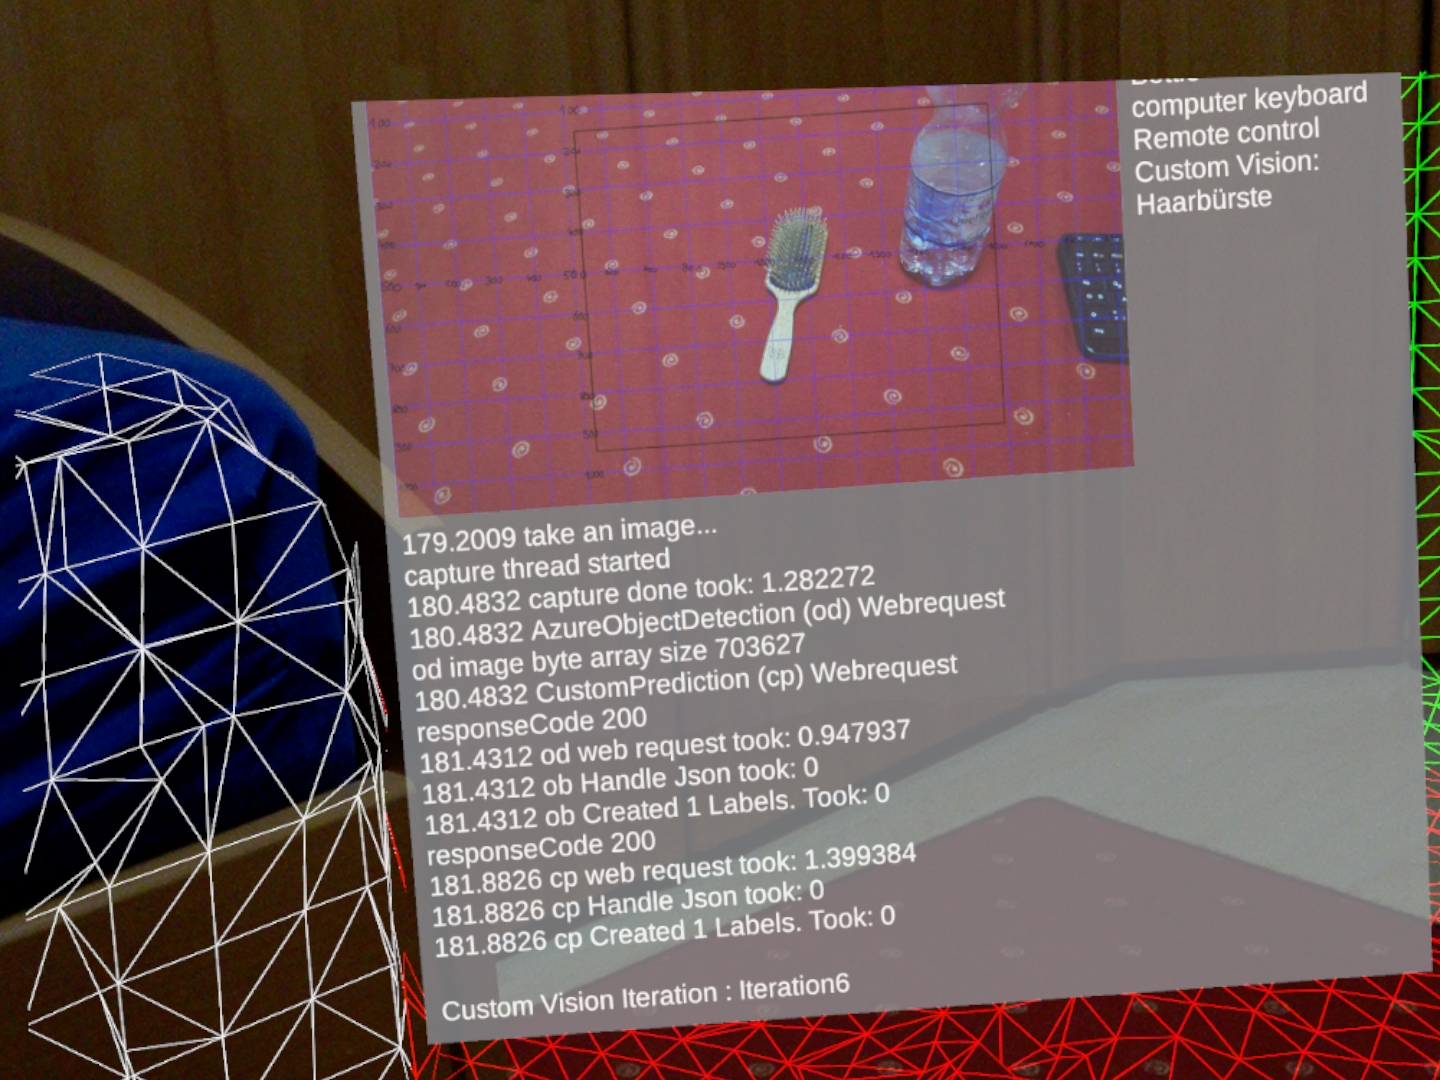
\includegraphics[width=0.75\textwidth]{images/ML_20201014_02.30.11.jpg}
	\caption[Laufzeit einer Objekterkennung]{Durchlauf mit Laufzeit Aufzeichnung}
	\label{img:laufzeit}
\end{figure}

Bei der Auswertung von 13 aufgenommenen Fotos wird festgestellt, dass Fotoaufnahmen durchschnittlich 1,11 Sekunden dauern. Inklusive Netzwerk Delay dauern Anfragen an Azure Object Detection durchschnittlich 0,96 Sekunden. Abzüglich des durchschnittlichen Netzwerk-Delays von 0,18 Sekunden ergibt sich eine durchschnittliche Analysezeit von 0,78 Sekunden. 

Inklusive Netzwek Delay dauern bei Iteration 6 Anfragen an Azure Custom Vision  durchschnittlich 1,84 Sekunden. Abzüglich des durchschnittlichen Netzwerk-Delays von 0,18 Sekunden ergibt sich somit eine durchschnittliche Analysezeit von 1,66 Sekunden.

Objekterkennungen mithilfe von Azure Object Detection und Azure Custom Vision werden parallel zueinander in unterschiedlichen Threads ausgeführt. Daher addieren sich ihre Laufzeiten nicht. Dementsprechend liegt die durchschnittliche Gesamtlaufzeit einer automatischen AR-Objekterkennung bei 2,95 Sekunden.

Das Auslesen der Json Antworten, das Lokalisieren der Objekte in der 3D-Szene und die Lable-Erstellung, benötigt weniger als eine Mikrosekunde. Siehe Abbildung \ref{table:laufzeitanalyse} und \ref{table:laufzeitanalyse2}.

\begin{figure}[H]
	\centering
	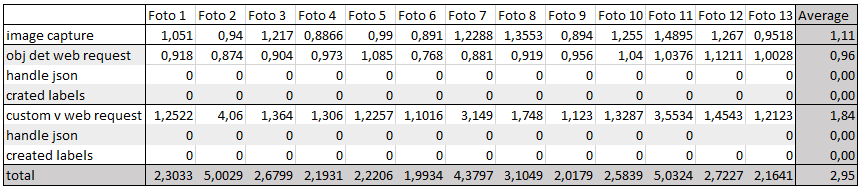
\includegraphics[width=1.1\textwidth]{images/table_Laufzeitanalyseneu.PNG}
	\caption[Laufzeitanalyse über 13 Bild-Analysen]{Laufzeitanalyse über 13 Bild-Analysen.}
	\label{table:laufzeitanalyse}
\end{figure}

\begin{figure}[H]
	\centering
	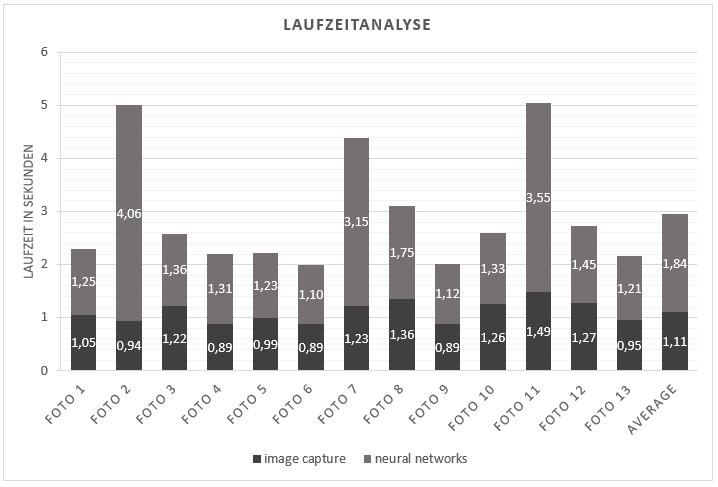
\includegraphics[width=0.95\textwidth]{images/table_Laufzeitanalyse2neu.PNG}
	\caption[Diagramm Laufzeitanalyse]{Diagramm Laufzeitanalyse}
	\label{table:laufzeitanalyse2}
\end{figure}

Da die Fotoaufnahme und die Anfragen an die Objekterkennungsservices zu lange dauern, ist es nicht möglich, die automatische Objekterkennung in Echtzeit durchzuführen. Die Verwendung eines einzigen neuronalen Netzwerkes würde die Laufzeit dieses Arbeitsschrittes verringern. Allerdings würde damit die Möglichkeit verloren gehen, mehrere neuronale Netze zu verwenden, um unterschiedliche Computer Vision Aufgaben erledigen zu können. Aus einem RGB-Bild können beispielsweise mehr semantische Informationen extrahiert werden, wenn Image Segmentation und Object Detection kombiniert werden. Daher kommt die Verwendung eines einziges neuronalen Netzwerkes nicht in Frage. Stattdessen wird dem Problem, dass die AR-Objekterkennung nicht echtzeitfähig ist, folgendermaßen begegnet: Die Resultate der Objekterkennungen werden in der Szene abgespeichert. Auf diese Weise können die semantischen Informationen in Echtzeit abgerufen werden, sobald sie benötigt sind.

Neben den Objekterkennung-Prozessen braucht das Aufnehmen der Fotos mit durchschnittlich 0.9 Sekunden einen signifikanten Teil der Gesamtlaufzeit. Durch einen Umstieg von Fotos auf Frames eines Videostreams ist es prinzipiell möglich, die Aufnahmezeit zu reduzieren. Dies kann in einer weiterführenden Arbeit umgesetzt werden. 
\subsection{Evaluierung der Objekterkennung durch Azure Objekt Detection}

Die Anwendung wird in einem Schlaf- und Arbeitszimmer getestet. Durch Azure Object Detection werden bei dem Test folgende Object-Klassen erkannt: Television, Person, Bottle, Keyboard, Computermouse, Cat, Bed, Luggage, Chair und Laptop.

Es stellt sich folgendes heraus: Azure Object Detection erkennt die Objekte mit unterschiedlicher Verlässlichkeit. Tastaturen und Personen werden in den meisten Aufnahmen korrekt erkannt. Das Lightwear-Gerät der 'Magic Leap One' wird gelegentlich als Computermaus interpretiert. Computerbildschirme werden durchweg als Television oder als Laptop markiert.

\subsection{Evaluierung der Objekterkennung durch Azure Custom Vision}

Die Genauigkeit der Objekterkennungen durch Azure Custom Vision hängt von dem Training des Modells ab. Azure Custom Vision erweist sich als effektive Ergänzung zur Azure Object Detection. Mithilfe der Iteration 6, wird das Objekt 'Haarbürste' zuverlässig erkannt. Dies ist auf das markante Aussehen des Objektes, die lange Testzeit von einer Stunde und die Verwendung von 51 Bildern zurückzuführen.

Für Bild-Regionen, in denen sich keine Haarbürste befindet, berechnet das Modell lediglich eine Probability von weniger als 5 Prozent dafür, dass sich dort eine Haarbürste befinden könnte. Regionen, die mit einer Probability von über 50 Prozent markiert werden, beinhalteten in der Anwendung tatsächlich zuverlässig eine Haarbürste.

Durch die niedrige Rate an false positives kann die Akzeptanzschwelle auf 60 Prozent gesetzt werden. Auf diese Weise wird die Rate der false negatives verringert. Dadurch wird die Haarbüste fast immer korrekt erkannt, wenn sie sich auf einem Bild befindet.

\subsection{Objekte in 3D-Szene lokalisieren}

In diesem Teil wird evaluiert, wie akkurat Foto-Objekte in der 3D-Umgebung lokalisiert und markiert werden.
Um die Lokalisierung zu evaluieren, werden RGB-Bilder zwischengespeichert, welche zur Objekterkennung genutzt werden. Auf den RGB-Bildern wird der Mittelpunkt der Bounding-Boxen markiert. Siehe Abbildung \ref{img:markedonimage}. Die Labels, welche in der Szene gesetzt werden, sollen mit diesen Positionen korrespondieren.
Es lässt sich beobachten, dass die Positionen der Labels um weniger als 2 cm von der idealen Position abweichen. Siehe Abbildung \ref{img:labelsszene}. 
\begin{figure}[H]
	\centering
	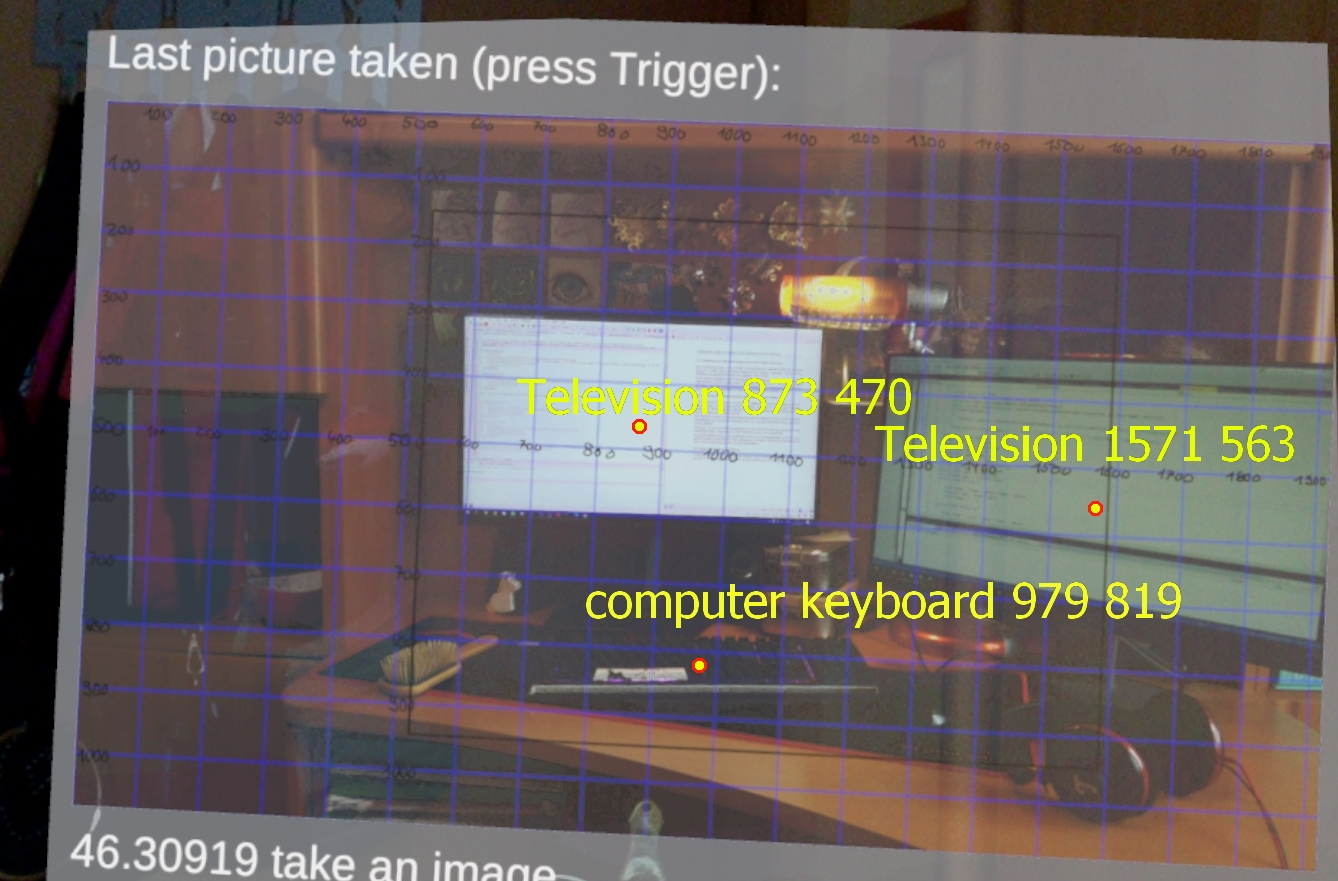
\includegraphics[width=0.7\textwidth]{images/ML_markedOnImage2.jpg}
	\caption[Erkennt Objekte auf RGB-Bilde markiert]{Die Mittelpunkte der erkannten Objekte werden, sind auf dem Foto per Hand markiert. Die Klassen und die u,v Foto-Koordinaten der Objekte sind angegeben.}
	\label{img:markedonimage}
\end{figure}

\begin{figure}[H]
	\centering
	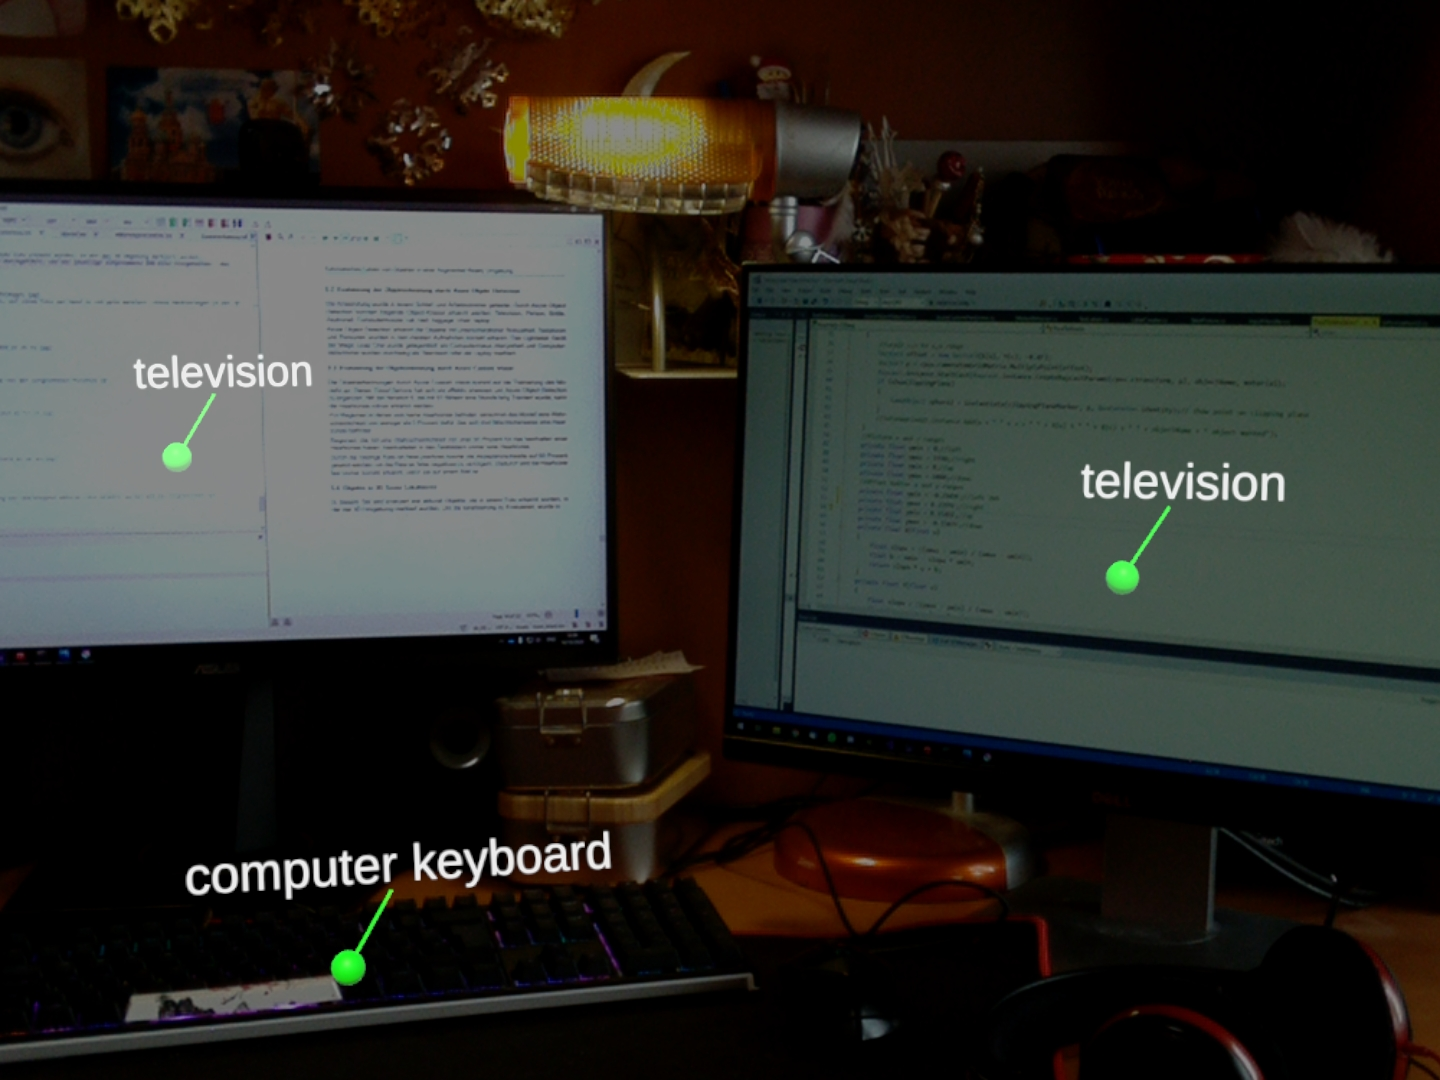
\includegraphics[width=0.7\textwidth]{images/ML_20201014_13.39.00.jpg}
	\caption[Erkannte Objekte in der Szene markiert]{In der 3D-Szene markierte Objekte.}
	\label{img:labelsszene}
\end{figure}

Die Lokalisierung der Objekte hängt von dem geometrischen Verständnis der AR-Brille ab. Objekte, die häufig bewegt werden, wie beispielsweise ein Stuhl, werden erst in die Spatial Map eingefügt, wenn sie über längere Zeit statisch bleiben. Das Einfügen des Objektes in die Map dauert ca. 2 Minuten. 

Wenn ein Objekt auf einem Foto erkannt wird und die Spatial Map an der Position des Gegenstandes fehlerhaft oder veraltet ist, wird das Objekt nicht korrekt markiert. Im vorliegenden Beispiel wird ein Stuhl auf einem Foto erkannt. Da der Stuhl kürzlich bewegt wurde, ist er jedoch nur bruchstückhaft in der Spatial Map vorhanden. Dies hat zur Folge, dass der Raycast bei Lokalisierung des Objektes durch den tatsächlichen Stuhl durchschießt. Der Raycast trifft stattdessen den Boden hinter dem Objekt und markiert diesen. Somit wird der Stuhl zwar korrekt durch die Objekterkennung erfasst, jedoch nicht korrekt in der Szene markiert. Siehe Abbildung \ref{img:stuhl}. 

\begin{figure}[H]
	\centering
	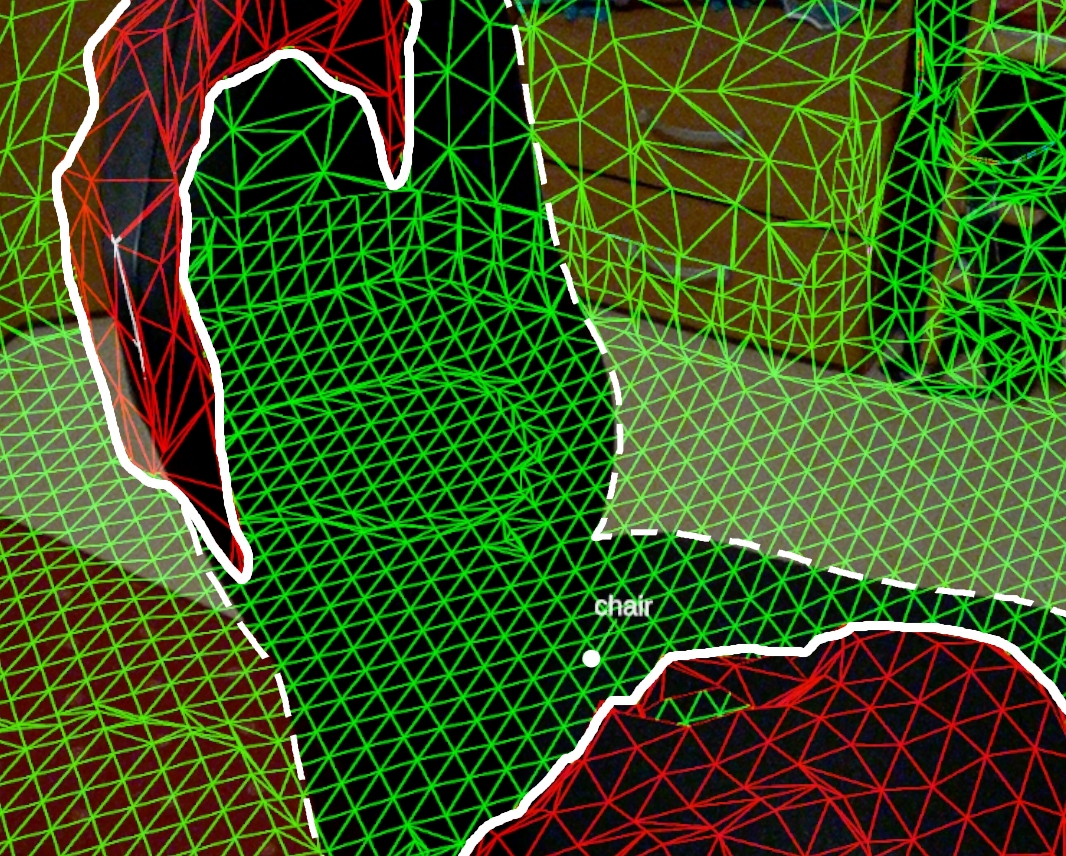
\includegraphics[width=0.65\textwidth]{images/ML_20201004_19.18.02_sup.jpg}
	\caption[Label setzen, bei fehlerhafter Spatial Map]{Spatial Map des Stuhles mit breiter Linie umrandet. Tatsächlicher Stuhl mit durchgebrochener Linie umrandet. Label des Stuhls markiert. Das Label befindet sich in der Szene hinter dem Stuhl auf dem Boden.}
	\label{img:stuhl}
\end{figure}

Halb transparente Objekte werden ebenfalls nicht korrekt in die Spatial Map eingefügt. In folgendem Beispiel wird das Label eines Flaschen-Objekts nicht korrekt positioniert: % Siehe Abbildung \ref{img:flasche}.

\begin{figure}[H]
	\centering
	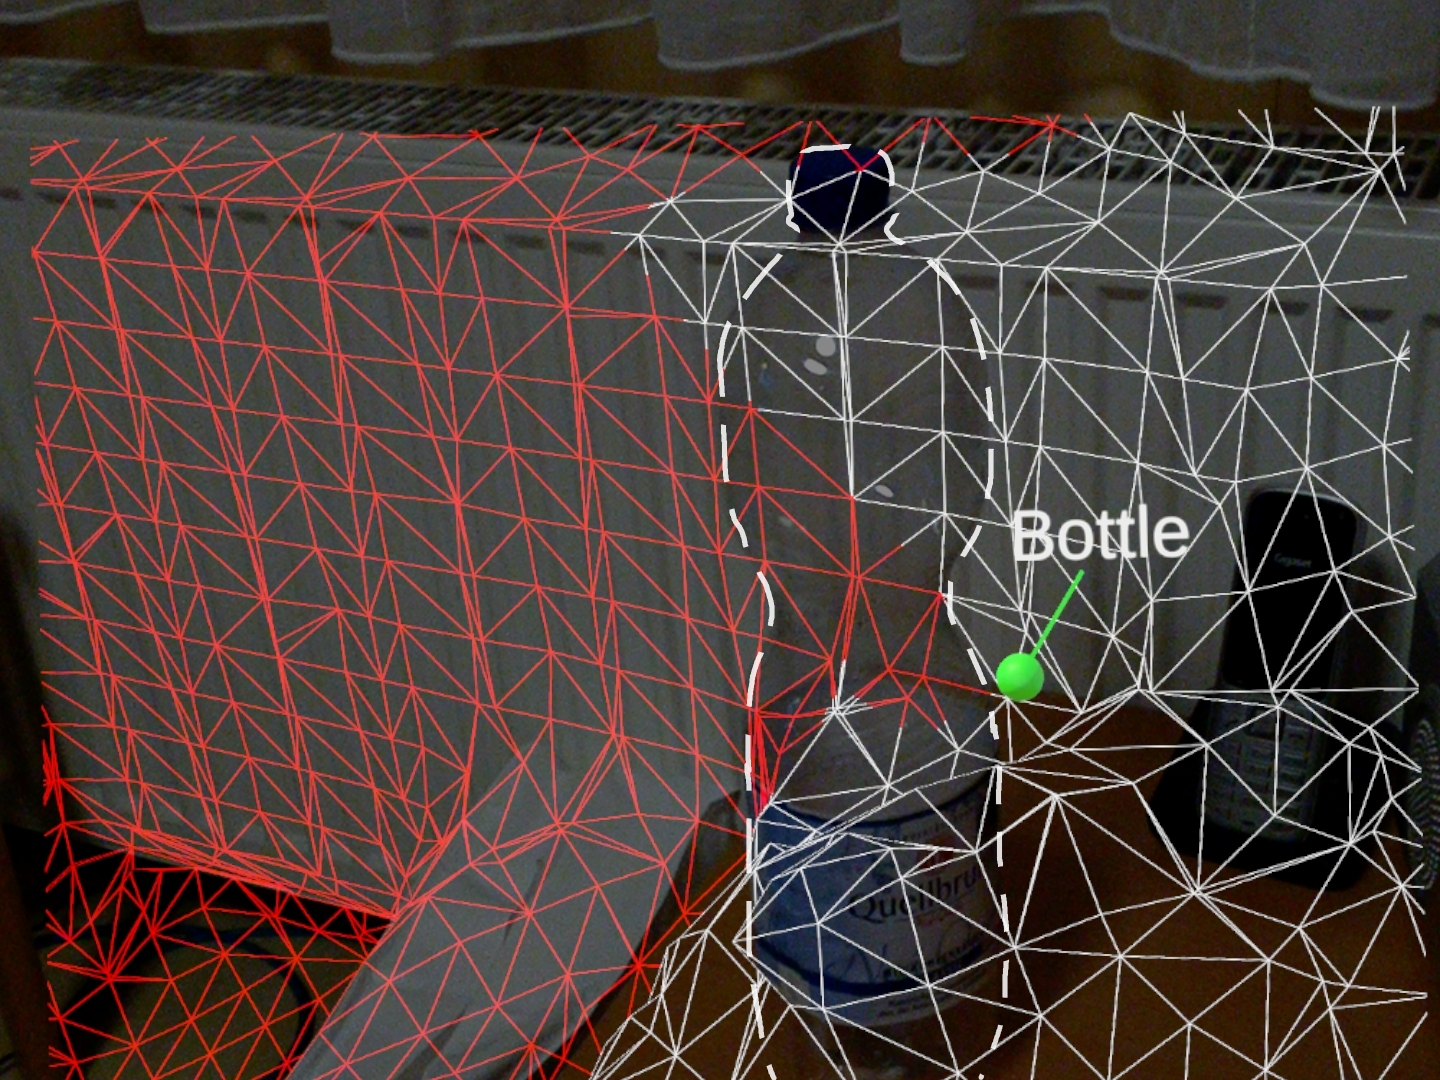
\includegraphics[width=0.65\textwidth]{images/ML_20201004_19.12.13_2.jpg}
	\caption[Spatial Mapping transparenter Objekte]{Das Label der Flasche liegt hinter dem tatsächlichen Objekt, da die Flasche nicht korrekt gemapped wurde.}
	\label{img:flasche}
\end{figure}
